%! Unidad 5 — Nomenclatura de química inorgánica (teoría, ejemplos resueltos, ejercicios por apartados, lectura, prácticas y
%! situación de aprendizaje)
%! Fuente: Fuentes/Quimica/Unidad 5 (capturas 527-539 y solucionario). Texto reescrito; compuestos de los ejercicios cambiados.
%! Normas: recomendaciones IUPAC de 2005 (y las de la RSEQ para el español). «hidrogeno» sin tilde dentro de los nombres
%! de hidrógeno; cargas de los iones como «(2\nobreakdash--)»; ecuaciones de hidratos con \ch{CuSO4 * 5 H2O}.
%! Figuras en images/UD5/ (html/ + render.sh): secuencia_elementos, estados_oxidacion, tipos_compuestos, adicion_oxoacido.

\sloppy % nombres largos sin guiones (dihidrogeno(tetraoxidosulfato)...): se permite más espacio entre palabras (\fussy al final)

\section*{Para empezar: azúcar de Saturno, vitriolo verde y gas hediondo}
\addcontentsline{toc}{section}{Para empezar: azúcar de Saturno, vitriolo verde y gas hediondo}

Los alquimistas y los primeros químicos ponían nombre a las sustancias según su aspecto, su sabor, su olor o el lugar del que
procedían: el \textbf{azúcar de Saturno} era un compuesto de plomo (el metal que se asociaba al planeta Saturno) de sabor dulce
y muy tóxico; el \textbf{vitriolo verde}, unos cristales verdes que hoy llamamos sulfato de hierro(II) heptahidrato, y el
\textbf{gas hediondo}, el sulfuro de hidrógeno, que huele a huevos podridos. Con unas decenas de sustancias, aquel sistema
funcionaba. Hoy se conocen muchos millones de compuestos y sería imposible recordar un nombre caprichoso para cada uno.

Por eso la comunidad científica se ha puesto de acuerdo en unas \textbf{reglas} que permiten asignar a cada sustancia un
\textbf{nombre} y una \textbf{fórmula} claros, sin ambigüedad. La institución encargada de fijarlas es la \textbf{IUPAC} (Unión
Internacional de Química Pura y Aplicada), fundada en 1919. Basta con mirar las etiquetas de los productos de casa para encontrar
compuestos inorgánicos: la lejía contiene hipoclorito de sodio, \ch{NaClO}; el salfumán es una disolución de cloruro de
hidrógeno, \ch{HCl}; la pasta de dientes lleva fluoruro de sodio, \ch{NaF}, y los productos para subir el pH de las piscinas,
carbonato de sodio, \ch{Na2CO3}. En esta unidad aprenderás a nombrar y formular estas sustancias y muchas más.

%========================================================================================
\section{Recuerda de la ESO}\label{sec:ud5-eso}
%========================================================================================

\paragraph{Fórmula química.} Cada sustancia pura se representa con una \textbf{fórmula}: los \textbf{símbolos} indican qué
elementos la forman y los \textbf{subíndices}, en qué \textbf{proporción} se combinan. Hay varios tipos de fórmulas; fíjate en
las de la hidracina, un combustible de cohetes formado por nitrógeno e hidrógeno:
\begin{itemize}
    \item \textbf{Fórmula empírica}, \ch{NH2}: solo da la proporción más sencilla (dos átomos de H por cada átomo de N).
    \item \textbf{Fórmula molecular}, \ch{N2H4}: da el número real de átomos de cada elemento en una molécula (2 de N y 4 de H).
    \item \textbf{Fórmula estructural}: muestra además cómo están unidos los átomos, por ejemplo:
    \[ \chemfig{H-N(-[2]H)-N(-[6]H)-H} \]
\end{itemize}

\paragraph{Valencia y estado de oxidación.} La \textbf{valencia} de un elemento está relacionada con el número de enlaces que
forma un átomo al combinarse. En Bachillerato usaremos casi siempre el \textbf{estado de oxidación}, un concepto parecido, pero no
idéntico, que lleva signo (sección~\ref{sec:ud5-conceptos}).

\paragraph{Nombrar y formular.} Un \textbf{sistema de nomenclatura} es un conjunto de reglas para nombrar las sustancias.
\textbf{Nombrar} es escribir el nombre a partir de la fórmula, y \textbf{formular}, escribir la fórmula a partir del nombre.

\paragraph{Prefijos multiplicadores.} Indican cuántos átomos o grupos hay de cada tipo. Los \textbf{simples} se usan con
átomos o grupos sencillos (\textit{di}óxido de carbono) y los \textbf{complejos}, con grupos cuyo nombre ya contiene un prefijo
o que podrían confundirse (\textit{bis}(trioxidonitrato) de calcio).

\begin{table}[H]
    \centering
    \caption{Prefijos multiplicadores}
    \vspace{-5pt}
    \begin{tabular}{@{}ccc@{\hspace{1.2cm}}ccc@{}}
        \toprule
        \textbf{Número} & \textbf{Simple} & \textbf{Complejo} & \textbf{Número} & \textbf{Simple} & \textbf{Complejo} \\
        \midrule
        1 & mono- & --- & 6 & hexa- & hexakis- \\[3pt]
        2 & di- & bis- & 7 & hepta- & heptakis- \\[3pt]
        3 & tri- & tris- & 8 & octa- & octakis- \\[3pt]
        4 & tetra- & tetrakis- & 9 & nona- & nonakis- \\[3pt]
        5 & penta- & pentakis- & 10 & deca- & decakis- \\
        \bottomrule
    \end{tabular}
    \label{tab:ud5-prefijos}
\end{table}

\begin{exercise}
    a) La fórmula molecular del peróxido de hidrógeno es \ch{H2O2}. ¿Cuál es su fórmula empírica? b) La del benceno es
    \ch{C6H6}. ¿Cuál es su fórmula empírica? c) ¿Puede una fórmula empírica coincidir con la molecular? Pon un ejemplo.
    \begin{solu}
        a) \textcolor{red}{\ch{HO}}. b) \textcolor{red}{\ch{CH}}. c) \textcolor{red}{Sí}, cuando los subíndices de la molecular
        ya no se pueden simplificar: \ch{H2O}, \ch{CO2}, \ch{NH3}\dots
    \end{solu}
\end{exercise}

%========================================================================================
\section{Conceptos previos}\label{sec:ud5-conceptos}
%========================================================================================

Para elaborar esta unidad seguimos las \textbf{recomendaciones de la IUPAC de 2005}, que son las vigentes, y las adaptaciones al
español de la Real Sociedad Española de Química. El nombre elegido para un compuesto debe identificarlo \textbf{sin ambigüedad}; se
evita la información redundante y se da prioridad a los nombres que no exigen conocer la estructura de la sustancia.

\subsection{Clasificación de las sustancias}

Las sustancias inorgánicas se clasifican según el \textbf{número de elementos distintos} que las forman
(figura~\ref{fig:ud5-tipos}):
\begin{itemize}
    \item \textbf{Sustancias simples} o elementos: un solo elemento (\ch{O2}, \ch{Fe}).
    \item \textbf{Compuestos binarios}: dos elementos (\ch{H2O}, \ch{NaCl}).
    \item \textbf{Compuestos ternarios}: tres elementos (\ch{H2SO4}, \ch{NaOH}).
    \item \textbf{Compuestos cuaternarios}: cuatro elementos (\ch{KHCO3}).
\end{itemize}

\begin{figure}[H]
    \centering
    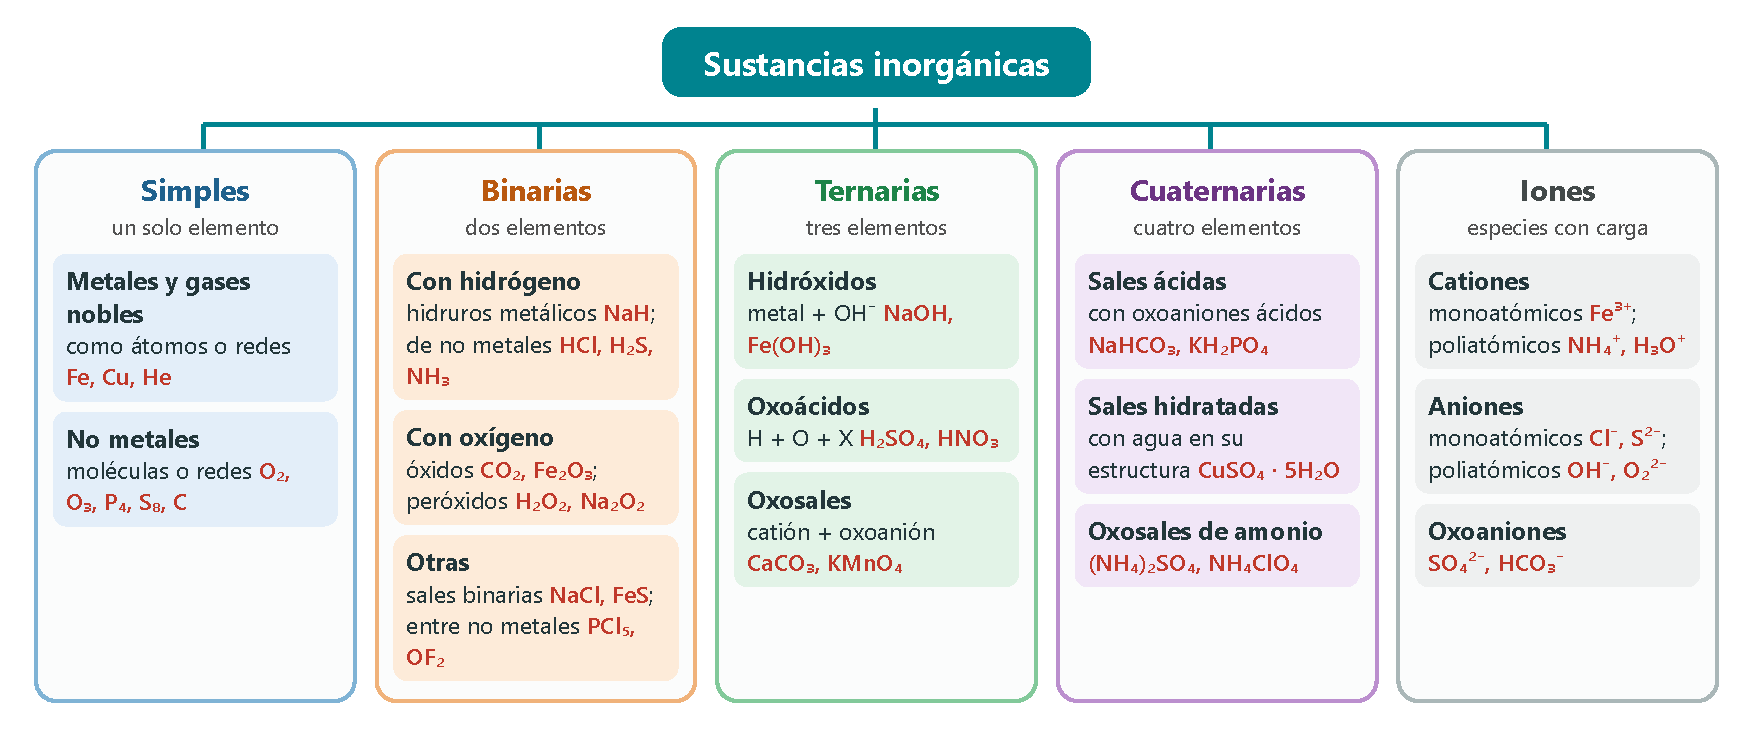
\includegraphics[width=\textwidth]{images/UD5/tipos_compuestos}
    \caption{Clasificación de las sustancias inorgánicas que estudiaremos en esta unidad, con algunos ejemplos.}
    \label{fig:ud5-tipos}
\end{figure}

\subsection{Número de carga y estado de oxidación}

\begin{definition}[Número de carga]
    Es la \textbf{carga eléctrica de un ion}. Se escribe con un número arábigo seguido del signo (\(+\) o \(-\)), entre
    paréntesis y justo detrás del nombre del ion, sin dejar espacio: el ion \ch{K+} es el ion potasio(1+) y el \ch{CO3^2-}, el ion
    trioxidocarbonato(2\nobreakdash--).
\end{definition}

El número de carga solo se puede usar para nombrar \textbf{compuestos iónicos}, que están formados por iones.

\begin{definition}[Estado de oxidación]
    Es la carga que tendría un átomo si todos sus enlaces fueran iónicos, es decir, si los electrones de cada enlace se los
    quedara por completo el átomo más electronegativo. Es positivo si el átomo «pierde» electrones y negativo si los «gana».
\end{definition}

El estado de oxidación se usa en las fórmulas y en los nombres como \textbf{número de oxidación}: un número romano, entre
paréntesis y sin espacio, detrás del nombre del elemento. Así, \ch{FeCO3} es el carbonato de hierro(II). En la
figura~\ref{fig:ud5-estados} tienes los estados de oxidación más frecuentes; algunos conviene saberlos de memoria:
\begin{itemize}
    \item Grupo 1 (alcalinos) y plata: \(+1\). Grupo 2 (alcalinotérreos), cinc y cadmio: \(+2\). Aluminio: \(+3\).
    \item Flúor: \(-1\). Oxígeno: \(-2\), salvo en los peróxidos (\(-1\)) y cuando se combina con el flúor.
    \item Hidrógeno: \(+1\) cuando se une a no metales y \(-1\) cuando se une a metales.
    \item Los elementos sin combinar (\ch{Fe}, \ch{O2}, \ch{P4}…) tienen estado de oxidación \textbf{cero}.
\end{itemize}

\begin{figure}[H]
    \centering
    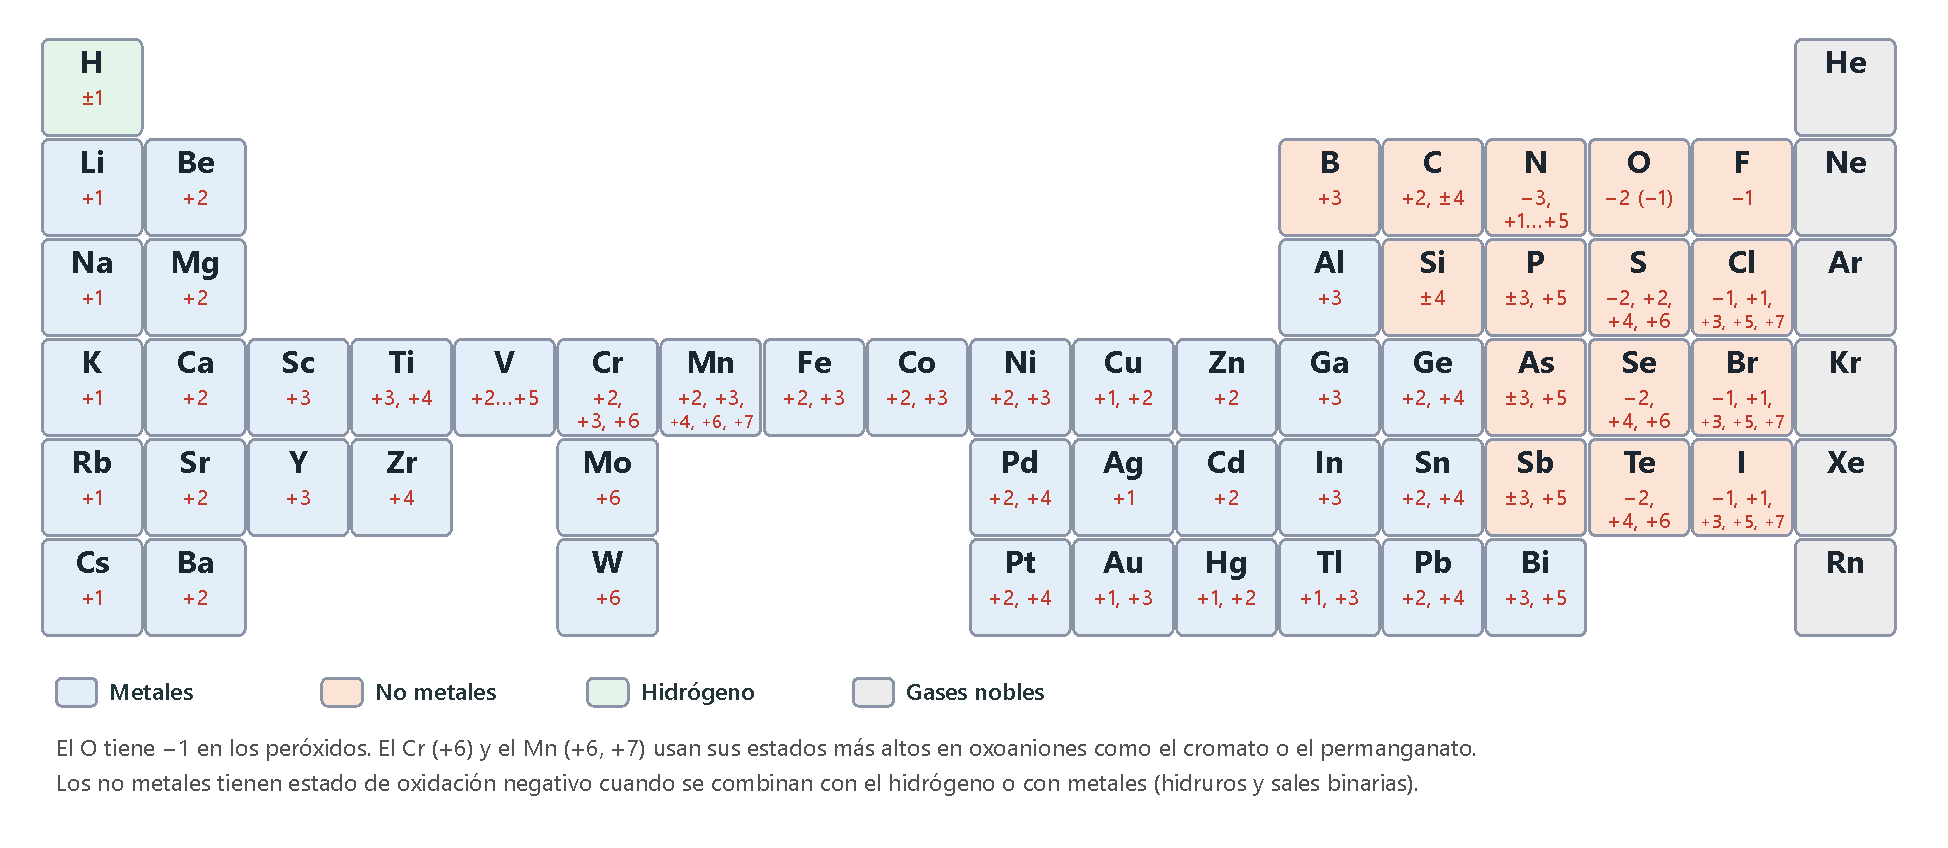
\includegraphics[width=\textwidth]{images/UD5/estados_oxidacion}
    \caption{Estados de oxidación más frecuentes de los elementos que usaremos en la unidad.}
    \label{fig:ud5-estados}
\end{figure}

\subsection{La regla de la suma}

\begin{definition}[Regla de la suma]
    En un compuesto \textbf{neutro}, la suma de los estados de oxidación de todos sus átomos (o de los números de carga de todos
    sus iones) es \textbf{cero}. En un \textbf{ion}, esa suma es igual a la \textbf{carga del ion}.
\end{definition}

Con esta regla y unos pocos valores memorizados puedes calcular el estado de oxidación de cualquier elemento en cualquier
compuesto.

\begin{example}
    \textbf{Calcular estados de oxidación.} Calcula el estado de oxidación del cromo en el \ch{K2Cr2O7}, del manganeso en el
    \ch{KMnO4}, del azufre en el \ch{Na2S2O3} y del nitrógeno en el ion \ch{NH4+}.

    \textbf{Solución.} Llamamos \(x\) al estado de oxidación desconocido y aplicamos la regla de la suma (K y Na, \(+1\);
    O, \(-2\); H, \(+1\)):
    \begin{itemize}
        \item \ch{K2Cr2O7}: \(2 \cdot (+1) + 2x + 7 \cdot (-2) = 0 \;\Rightarrow\; 2x = 12 \;\Rightarrow\; x = +6\).
        \item \ch{KMnO4}: \(+1 + x + 4 \cdot (-2) = 0 \;\Rightarrow\; x = +7\).
        \item \ch{Na2S2O3}: \(2 \cdot (+1) + 2x + 3 \cdot (-2) = 0 \;\Rightarrow\; 2x = 4 \;\Rightarrow\; x = +2\).
        \item \ch{NH4+}: \(x + 4 \cdot (+1) = +1 \;\Rightarrow\; x = -3\) (la suma es la carga del ion, no cero).
    \end{itemize}
\end{example}

\begin{exercise}
    Calcula el estado de oxidación del elemento destacado en negrita: a) \textbf{S} en \ch{H2SO3}; b) \textbf{P} en \ch{Ca3(PO4)2};
    c) \textbf{Cl} en \ch{ClO4-}; d) \textbf{C} en \ch{CH4}; e) \textbf{Fe} en \ch{Fe2O3}; f) \textbf{N} en \ch{NO2-}; g)
    \textbf{O} en \ch{BaO2}; h) \textbf{Cr} en \ch{CrO4^2-}.
    \begin{solu}
        a) \(2 + x - 6 = 0\): \textcolor{red}{\(+4\)}. b) El fosfato es \ch{PO4^3-}: \(x - 8 = -3\): \textcolor{red}{\(+5\)}.
        c) \(x - 8 = -1\): \textcolor{red}{\(+7\)}. d) \(x + 4 = 0\): \textcolor{red}{\(-4\)}. e) \(2x - 6 = 0\):
        \textcolor{red}{\(+3\)}. f) \(x - 4 = -1\): \textcolor{red}{\(+3\)}. g) \(2 + 2x = 0\): \textcolor{red}{\(-1\)} (es un
        peróxido). h) \(x - 8 = -2\): \textcolor{red}{\(+6\)}.
    \end{solu}
\end{exercise}

\begin{exercise}
    Usando la regla de la suma, indica si son posibles estas fórmulas y, si no lo son, corrígelas: a) \ch{CaCl}; b) \ch{Al2O3};
    c) \ch{KS}; d) \ch{Ba3N2}; e) \ch{LiO}; f) \ch{MgF2}.
    \begin{solu}
        a) \(+2 - 1 \neq 0\): \textcolor{red}{no; \ch{CaCl2}}. b) \(2 \cdot 3 + 3 \cdot (-2) = 0\): \textcolor{red}{sí}.
        c) \(+1 - 2 \neq 0\): \textcolor{red}{no; \ch{K2S}}. d) \(3 \cdot 2 + 2 \cdot (-3) = 0\): \textcolor{red}{sí}.
        e) \(+1 - 2 \neq 0\): \textcolor{red}{no; \ch{Li2O}}. f) \(+2 + 2 \cdot (-1) = 0\): \textcolor{red}{sí}.
    \end{solu}
\end{exercise}

\subsection{La secuencia de los elementos}

Al escribir una fórmula hay que colocar los símbolos en un \textbf{orden determinado}. La IUPAC ha fijado por convenio una
\textbf{secuencia de los elementos} (figura~\ref{fig:ud5-secuencia}): se recorre la tabla periódica empezando por los gases nobles
y avanzando grupo a grupo, de abajo arriba dentro de cada grupo, con el hidrógeno colocado entre los grupos 15 y 16, hasta terminar
en el flúor.

\begin{definition}[Orden en la fórmula]
    De dos elementos, se escribe a la \textbf{izquierda} el que aparece \textbf{antes} en la secuencia, que hace el papel de
    \textbf{electropositivo}, y a la \textbf{derecha} el que aparece \textbf{después}, que hace el papel de
    \textbf{electronegativo}.
\end{definition}

\begin{figure}[H]
    \centering
    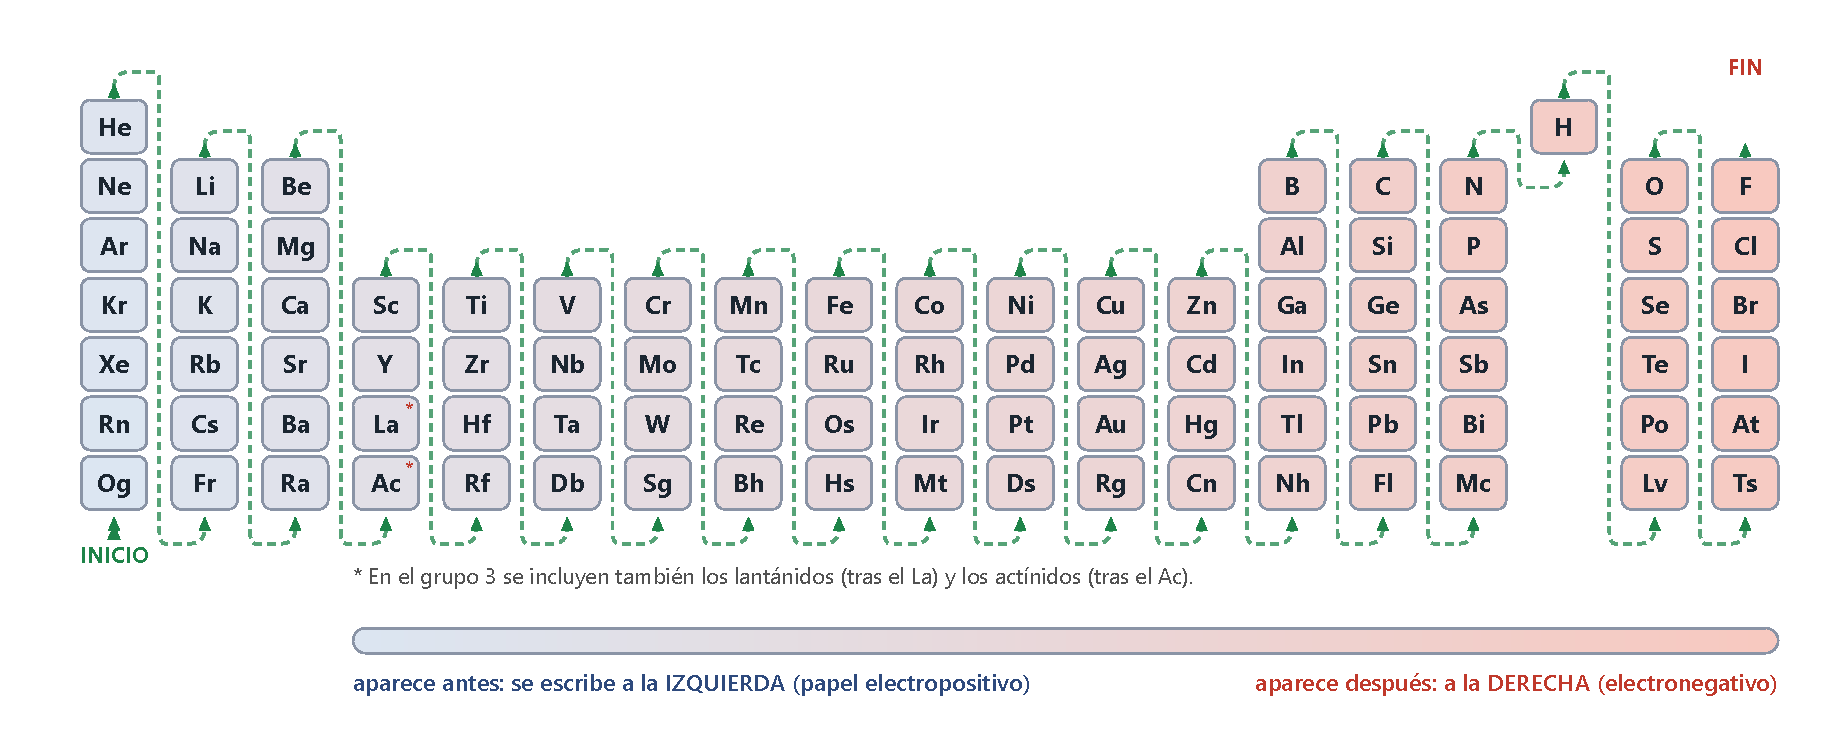
\includegraphics[width=\textwidth]{images/UD5/secuencia_elementos}
    \caption{Secuencia de los elementos para formular y nombrar (IUPAC 2005). Se avanza de abajo arriba en cada grupo y de un
    grupo al siguiente siguiendo las flechas.}
    \label{fig:ud5-secuencia}
\end{figure}

Esta secuencia se parece mucho a ordenar los elementos por su electronegatividad, que era el criterio antiguo, pero no es igual.
Por ejemplo, el oxígeno aparece antes que los halógenos: la fórmula es \ch{OCl2} y no \ch{Cl2O}. En el amoniaco, el nitrógeno va
antes que el hidrógeno (\ch{NH3}), y en el agua el hidrógeno va antes que el oxígeno (\ch{H2O}).

\subsection{Sistemas de nomenclatura}

La IUPAC recomienda tres sistemas de nomenclatura; además, acepta algunos nombres tradicionales.

\begin{table}[H]
    \centering
    \caption{Sistemas de nomenclatura}
    \vspace{-5pt}
    \begin{tabular}{@{}L{3.2cm}L{11cm}@{}}
        \toprule
        \textbf{Sistema} & \textbf{En qué consiste} \\
        \midrule
        De composición o estequiométrica & Se basa en la \textbf{composición}: indica los elementos y su proporción, pero no la
        estructura. La proporción se da con \textbf{prefijos multiplicadores} (dióxido de carbono), con el \textbf{número de
        oxidación} (óxido de carbono(IV)) o, solo en compuestos iónicos, con el \textbf{número de carga} (óxido de hierro(3+)). La
        única contracción admitida es monóxido: se escribe tetraóxido, pentaóxido (no «tetróxido», «pentóxido»). \\[3pt]
        De adición & Considera que el compuesto tiene un \textbf{átomo central} unido a otros átomos o grupos, los
        \textbf{ligandos}. No se usa para compuestos binarios. Es la base de los nombres de los oxoácidos. \\[3pt]
        De sustitución & Parte de un compuesto progenitor con nombre propio (el \textbf{hidruro progenitor}) y sustituye
        algunos de sus átomos de hidrógeno. Es la base de la química orgánica. \\[3pt]
        Nombres tradicionales & La IUPAC acepta unos pocos nombres muy extendidos que no siguen reglas sistemáticas: agua,
        amoniaco, ácido sulfúrico… \\[3pt]
        Nomenclatura de hidrógeno & Variante de la de adición para compuestos con hidrógeno cuya estructura no se conoce o no se
        quiere indicar: dihidrogeno(tetraoxidosulfato). \\
        \bottomrule
    \end{tabular}
    \label{tab:ud5-sistemas}
\end{table}

%========================================================================================
\section{Sustancias simples}\label{sec:ud5-simples}
%========================================================================================

\begin{definition}[Sustancia simple]
    Es la formada por átomos de un \textbf{mismo elemento}. Su estado de oxidación es siempre \textbf{cero}.
\end{definition}

\begin{itemize}
    \item Si la sustancia está formada por \textbf{átomos sueltos} (los gases nobles) o por \textbf{redes cristalinas} (los
    metales y algunos no metales, como el carbono o el silicio), se formula con el símbolo y se nombra con el nombre del
    elemento: \ch{He}, helio; \ch{Au}, oro; \ch{C}, carbono.
    \item Si está formada por \textbf{moléculas}, la fórmula lleva un \textbf{subíndice} con el número de átomos y el nombre
    lleva el \textbf{prefijo multiplicador} correspondiente: \ch{H2}, dihidrógeno; \ch{O3}, trioxígeno; \ch{P4}, tetrafósforo;
    \ch{S8}, octaazufre.
\end{itemize}

El prefijo \textit{mono} solo se usa si el elemento no se presenta de forma monoatómica en la naturaleza: \ch{N} es
mononitrógeno, una especie muy reactiva distinta del \ch{N2} del aire (dinitrógeno). La IUPAC acepta los nombres \textbf{oxígeno}
para el \ch{O2} y \textbf{ozono} para el \ch{O3}.

\begin{exercise}
    Nombra o formula: a) \ch{Ne}; b) \ch{Br2}; c) \ch{Ag}; d) \ch{S8}; e) \ch{F2}; f) \ch{O}; g) argón; h) cobre; i) ozono;
    j) dinitrógeno; k) tetrafósforo; l) diyodo.
    \begin{solu}
        a) \textcolor{red}{neón}; b) \textcolor{red}{dibromo}; c) \textcolor{red}{plata}; d) \textcolor{red}{octaazufre};
        e) \textcolor{red}{diflúor}; f) \textcolor{red}{monooxígeno}; g) \textcolor{red}{\ch{Ar}}; h) \textcolor{red}{\ch{Cu}};
        i) \textcolor{red}{\ch{O3}}; j) \textcolor{red}{\ch{N2}}; k) \textcolor{red}{\ch{P4}}; l) \textcolor{red}{\ch{I2}}.
    \end{solu}
\end{exercise}

%========================================================================================
\section{Iones}\label{sec:ud5-iones}
%========================================================================================

\begin{definition}[Ion]
    Es una especie química con carga eléctrica, porque ha \textbf{ganado} o \textbf{perdido} electrones. Si su carga es
    \textbf{negativa} se llama \textbf{anión}, y si es \textbf{positiva}, \textbf{catión}.
\end{definition}

\subsection{Iones monoatómicos}

Proceden de un solo átomo. Los estados de oxidación de la figura~\ref{fig:ud5-estados} te dicen qué iones son los más probables:
el potasio (\(+1\)) forma \ch{K+}; el hierro (\(+2\), \(+3\)), \ch{Fe^2+} y \ch{Fe^3+}, y el azufre, como no metal, tiende a
ganar electrones y formar \ch{S^2-}.

\paragraph{Formular.} Se escribe el símbolo y, como superíndice, la carga: primero el número y después el signo. El 1 no se
escribe: \ch{Cl-}, \ch{N^3-}, \ch{K+}, \ch{Fe^3+}.

\paragraph{Aniones monoatómicos.} Se nombran con la raíz del nombre del elemento terminada en \textbf{-uro} y, si hace falta, el
número de carga: \ch{N^3-} es nitruro(3\nobreakdash--), o simplemente \textbf{nitruro}, porque el nitrógeno solo forma un anión. Algunos
elementos usan la raíz latina: \ch{S^2-}, \textbf{sulfuro}. La excepción más importante es el \ch{O^2-}, que se llama
\textbf{óxido}.

\paragraph{Cationes monoatómicos.} Se nombran con el nombre del elemento seguido \textbf{siempre} del número de carga, aunque
sea único: \ch{K+} es el potasio(1+) y \ch{Fe^3+}, el hierro(3+).

\subsection{Iones poliatómicos}

\paragraph{Homopoliatómicos.} Están formados por varios átomos de un \textbf{mismo elemento}. Se nombran con prefijos
multiplicadores, y el número de átomos se escribe como subíndice. Algunos tienen nombres no sistemáticos aceptados por la IUPAC.

\begin{table}[H]
    \centering
    \caption{Iones poliatómicos frecuentes}
    \vspace{-5pt}
    \begin{tabular}{@{}lL{4.6cm}@{\hspace{1cm}}lL{4.6cm}@{}}
        \toprule
        \textbf{Fórmula} & \textbf{Nombre} & \textbf{Fórmula} & \textbf{Nombre} \\
        \midrule
        \ch{Hg2^2+} & dimercurio(2+) & \ch{O2^2-} & dióxido(2\nobreakdash--) o \textbf{peróxido} \\[3pt]
        \ch{I3-} & triyoduro(1\nobreakdash--) & \ch{C2^2-} & dicarburo(2\nobreakdash--) o \textbf{acetiluro} \\[3pt]
        \ch{NH4+} & azanio o \textbf{amonio} & \ch{OH-} & hidróxido \\[3pt]
        \ch{H3O+} & oxidanio u \textbf{oxonio} & \ch{CN-} & cianuro \\
        \bottomrule
    \end{tabular}
    \label{tab:ud5-poliatomicos}
\end{table}

\paragraph{Heteropoliatómicos.} Tienen \textbf{más de un elemento}. Los más importantes son los \textbf{oxoaniones}, como el
\ch{CO3^2-}, que estudiaremos en la sección~\ref{sec:ud5-oxoaniones}. Los cuatro de la tabla~\ref{tab:ud5-poliatomicos} (amonio,
oxonio, hidróxido y cianuro) conviene aprenderlos ya. Fíjate en que en el \ch{OH-} los símbolos no siguen la secuencia de los
elementos: es una excepción aceptada.

\begin{exercise}
    Nombra o formula estos iones: a) \ch{Br-}; b) \ch{Ca^2+}; c) \ch{Se^2-}; d) \ch{Cu+}; e) \ch{P^3-}; f) \ch{H3O+};
    g) \ch{Co^3+}; h) \ch{O2^2-}; i) yoduro; j) óxido; k) estaño(4+); l) amonio; m) hidróxido; n) plata(1+); ñ) fluoruro; o)
    mercurio(2+).
    \begin{solu}
        a) \textcolor{red}{bromuro}; b) \textcolor{red}{calcio(2+)}; c) \textcolor{red}{seleniuro}; d) \textcolor{red}{cobre(1+)};
        e) \textcolor{red}{fosfuro}; f) \textcolor{red}{oxonio (oxidanio)}; g) \textcolor{red}{cobalto(3+)}; h)
        \textcolor{red}{peróxido (dióxido(2\nobreakdash--))}; i) \textcolor{red}{\ch{I-}}; j) \textcolor{red}{\ch{O^2-}}; k)
        \textcolor{red}{\ch{Sn^4+}}; l) \textcolor{red}{\ch{NH4+}}; m) \textcolor{red}{\ch{OH-}}; n) \textcolor{red}{\ch{Ag+}};
        ñ) \textcolor{red}{\ch{F-}}; o) \textcolor{red}{\ch{Hg^2+}}.
    \end{solu}
\end{exercise}

%========================================================================================
\section{Compuestos binarios}\label{sec:ud5-binarios}
%========================================================================================

\begin{definition}[Compuesto binario]
    Es el formado por átomos de \textbf{dos elementos} diferentes. Se nombran con la nomenclatura de \textbf{composición} (y
    los hidruros de los grupos 13 a 17, también con la de \textbf{sustitución}).
\end{definition}

\paragraph{Formular.} El elemento que aparece \textbf{antes} en la secuencia (figura~\ref{fig:ud5-secuencia}) se escribe a la
\textbf{izquierda} y hace de \textbf{electropositivo}; el otro, a la derecha, hace de \textbf{electronegativo} y tiene estado de
oxidación negativo. Los \textbf{subíndices} se deducen de la \textbf{neutralidad}: la suma de los estados de oxidación (o de los
números de carga) tiene que ser cero.

\paragraph{Nombrar.} Se lee la fórmula de \textbf{derecha a izquierda}: primero el elemento electronegativo, con la terminación
\textbf{-uro} (u \textbf{óxido} si es el oxígeno), después «de» y el nombre del elemento electropositivo. La proporción se
indica de una de estas formas:
\begin{itemize}
    \item Con \textbf{prefijos multiplicadores} en los dos elementos: \ch{CaF2} es difluoruro de calcio. El prefijo
    \textit{mono} se puede omitir, salvo en monóxido.
    \item Con el \textbf{número de oxidación} del electropositivo: fluoruro de calcio(II).
    \item Con el \textbf{número de carga} del catión, solo si el compuesto es iónico: fluoruro de calcio(2+).
\end{itemize}
El número de oxidación o de carga solo se indica en el elemento electropositivo, y se puede \textbf{omitir} si ese elemento
solo tiene un estado de oxidación: \ch{CaF2} es, sencillamente, \textbf{fluoruro de calcio}.

\begin{example}
    \textbf{Formular un binario.} Formula el compuesto de calcio y flúor y nómbralo de todas las formas posibles.

    \textbf{Solución.} \textbf{1. Orden}: el calcio aparece antes que el flúor en la secuencia: \ch{Ca} a la izquierda y
    \ch{F} a la derecha. \textbf{2. Estados de oxidación}: \(\ch{Ca} = +2\) (su único valor) y \(\ch{F} = -1\).
    \textbf{3. Neutralidad}: \(1 \cdot (+2) + 2 \cdot (-1) = 0\): hacen falta dos átomos de F por cada átomo de Ca, y la fórmula
    es \ch{CaF2}. \textbf{4. Nombres}: difluoruro de calcio; fluoruro de calcio(II); fluoruro de calcio(2+), o simplemente
    \textbf{fluoruro de calcio}, porque el calcio solo tiene un estado de oxidación.
\end{example}

\subsection{Compuestos binarios con hidrógeno}\label{sec:ud5-hidruros}

La posición del hidrógeno en la fórmula depende del elemento con el que se combina.

\paragraph{Hidruros de los grupos 1 a 15.} El hidrógeno aparece después en la secuencia: se escribe a la \textbf{derecha}, hace
de electronegativo y tiene estado de oxidación \(-1\). Se nombran con la palabra \textbf{hidruro}, y la proporción se indica con
prefijos multiplicadores o con el número de oxidación del otro elemento, si tiene más de uno. Si el otro elemento es un metal, el
compuesto es iónico (contiene el ion hidruro, \ch{H-}) y también se puede usar el número de carga.

\paragraph{Hidruros de los grupos 16 y 17 (salvo el oxígeno).} El hidrógeno aparece antes en la secuencia: se escribe a la
\textbf{izquierda}, hace de electropositivo y tiene estado de oxidación \(+1\). Se nombran con el otro elemento terminado en
\textbf{-uro} seguido de «de hidrógeno». No son iónicos, así que no se usa el número de carga, y como el hidrógeno solo tiene un
estado de oxidación positivo, tampoco hace falta el número de oxidación. Sus \textbf{disoluciones acuosas} son ácidas y antes se
llamaban \textbf{ácidos hidrácidos} (ácido clorhídrico, ácido sulfhídrico): la IUPAC no acepta esos nombres para los compuestos
puros, porque son nombres de las disoluciones.

\begin{table}[H]
    \centering
    \caption{Nomenclatura de composición de algunos compuestos binarios con hidrógeno}
    \vspace{-5pt}
    \begin{tabular}{@{}lL{3.6cm}L{3.6cm}L{3.6cm}@{}}
        \toprule
        \textbf{Fórmula} & \textbf{Prefijos multiplicadores} & \textbf{Número de oxidación} & \textbf{Número de carga} \\
        \midrule
        \ch{CuH2} & dihidruro de cobre & hidruro de cobre(II) & hidruro de cobre(2+) \\[3pt]
        \ch{AlH3} & trihidruro de aluminio & hidruro de aluminio & hidruro de aluminio \\[3pt]
        \ch{NH3} & trihidruro de nitrógeno & hidruro de nitrógeno(III) & --- \\[3pt]
        \ch{CH4} & tetrahidruro de carbono & hidruro de carbono(IV) & --- \\[3pt]
        \ch{H2S} & sulfuro de dihidrógeno & sulfuro de hidrógeno & --- \\[3pt]
        \ch{HCl} & cloruro de hidrógeno & cloruro de hidrógeno & --- \\
        \bottomrule
    \end{tabular}
    \label{tab:ud5-hidruros}
\end{table}

\paragraph{Nomenclatura de sustitución.} Los hidruros de los grupos 13 a 17 son los \textbf{hidruros progenitores}, de los que
derivan muchos otros compuestos. Se nombran con la raíz del elemento y la terminación \textbf{-ano}. El agua y el amoniaco
mantienen sus nombres tradicionales, que son los recomendados.

\begin{table}[H]
    \centering
    \caption{Hidruros progenitores (nomenclatura de sustitución)}
    \vspace{-5pt}
    \begin{tabular}{@{}ll@{\hspace{0.8cm}}ll@{\hspace{0.8cm}}ll@{\hspace{0.8cm}}ll@{}}
        \toprule
        \multicolumn{2}{@{}c}{\textbf{Grupo 13 y 14}} & \multicolumn{2}{c}{\textbf{Grupo 15}} & \multicolumn{2}{c}{\textbf{Grupo
        16}} & \multicolumn{2}{c@{}}{\textbf{Grupo 17}} \\
        \midrule
        \ch{BH3} & borano & \ch{NH3} & azano, \textbf{amoniaco} & \ch{H2O} & oxidano, \textbf{agua} & \ch{HF} & fluorano \\[3pt]
        \ch{AlH3} & alumano & \ch{PH3} & fosfano & \ch{H2S} & sulfano & \ch{HCl} & clorano \\[3pt]
        \ch{CH4} & metano & \ch{AsH3} & arsano & \ch{H2Se} & selano & \ch{HBr} & bromano \\[3pt]
        \ch{SiH4} & silano & \ch{SbH3} & estibano & \ch{H2Te} & telano & \ch{HI} & yodano \\
        \bottomrule
    \end{tabular}
    \label{tab:ud5-progenitores}
\end{table}

De los progenitores derivan otras especies: el ion \ch{H3O+}, oxidanio, procede del oxidano (\ch{H2O}), y el \ch{NH4+}, azanio,
del azano (\ch{NH3}).

\begin{example}
    \textbf{Hidruros.} Nombra de todas las formas posibles: \ch{PbH4}, \ch{KH}, \ch{BH3}, \ch{H2Te} y \ch{GeH4}.

    \textbf{Solución.}
    \begin{itemize}
        \item \ch{PbH4}: tetrahidruro de plomo; hidruro de plomo(IV); hidruro de plomo(4+) (el plomo tiene \(+2\) y \(+4\): hay
        que indicarlo).
        \item \ch{KH}: hidruro de potasio (el potasio solo tiene \(+1\); con prefijos, monohidruro de potasio o hidruro de
        potasio).
        \item \ch{BH3}: trihidruro de boro; hidruro de boro; \textbf{borano}. No es iónico: no hay número de carga.
        \item \ch{H2Te}: telururo de dihidrógeno; telururo de hidrógeno; \textbf{telano}.
        \item \ch{GeH4}: tetrahidruro de germanio; hidruro de germanio(IV); \textbf{germano}.
    \end{itemize}
\end{example}

\begin{exercise}
    Nombra de todas las maneras posibles: a) \ch{NaH}; b) \ch{BaH2}; c) \ch{FeH3}; d) \ch{CoH2}; e) \ch{HBr}; f) \ch{H2Se};
    g) \ch{SnH4}; h) \ch{PH3}; i) \ch{AsH3}; j) \ch{HF}; k) \ch{AuH}; l) \ch{SiH4}.
    \begin{solu}
        a) \textcolor{red}{hidruro de sodio}. b) \textcolor{red}{dihidruro de bario; hidruro de bario}. c)
        \textcolor{red}{trihidruro de hierro; hidruro de hierro(III); hidruro de hierro(3+)}. d) \textcolor{red}{dihidruro de
        cobalto; hidruro de cobalto(II); hidruro de cobalto(2+)}. e) \textcolor{red}{bromuro de hidrógeno; bromano}. f)
        \textcolor{red}{seleniuro de dihidrógeno; seleniuro de hidrógeno; selano}. g) \textcolor{red}{tetrahidruro de estaño;
        hidruro de estaño(IV); hidruro de estaño(4+); estannano}. h) \textcolor{red}{trihidruro de fósforo; hidruro de
        fósforo(III); fosfano}. i) \textcolor{red}{trihidruro de arsénico; hidruro de arsénico(III); arsano}. j)
        \textcolor{red}{fluoruro de hidrógeno; fluorano}. k) \textcolor{red}{hidruro de oro; hidruro de oro(I); hidruro de
        oro(1+)}. l) \textcolor{red}{tetrahidruro de silicio; hidruro de silicio; silano}.
    \end{solu}
\end{exercise}

\begin{exercise}
    Formula: a) hidruro de litio; b) dihidruro de magnesio; c) hidruro de níquel(III); d) hidruro de cobre(1+); e) cloruro de
    hidrógeno; f) sulfuro de dihidrógeno; g) estibano; h) metano; i) hidruro de paladio(IV); j) yoduro de hidrógeno; k)
    trihidruro de cromo; l) azano.
    \begin{solu}
        a) \textcolor{red}{\ch{LiH}}; b) \textcolor{red}{\ch{MgH2}}; c) \textcolor{red}{\ch{NiH3}}; d) \textcolor{red}{\ch{CuH}};
        e) \textcolor{red}{\ch{HCl}}; f) \textcolor{red}{\ch{H2S}}; g) \textcolor{red}{\ch{SbH3}}; h) \textcolor{red}{\ch{CH4}};
        i) \textcolor{red}{\ch{PdH4}}; j) \textcolor{red}{\ch{HI}}; k) \textcolor{red}{\ch{CrH3}}; l) \textcolor{red}{\ch{NH3}}.
    \end{solu}
\end{exercise}

\subsection{Compuestos binarios con oxígeno}\label{sec:ud5-oxidos}

\paragraph{Óxidos.} Son las combinaciones binarias del oxígeno con cualquier elemento \textbf{excepto los halógenos}. Pueden ser
\textbf{metálicos} (\ch{Fe2O3}) o \textbf{no metálicos} (\ch{CO2}). El oxígeno se escribe a la \textbf{derecha} y tiene estado
de oxidación \(-2\).

\begin{itemize}
    \item \textbf{Nombrar}: con prefijos multiplicadores (dióxido de carbono; el \textit{mono} se puede omitir si no hay
    ambigüedad, pero no en el \ch{CO}, monóxido de carbono, para distinguirlo del \ch{CO2}); con el número de oxidación del
    otro elemento, calculado con la regla de la suma (en el \ch{CO2}, \(x + 2 \cdot (-2) = 0\), \(x = +4\): óxido de
    carbono(IV)), o, solo en los óxidos metálicos, que son iónicos, con el número de carga (\ch{Fe2O3}, óxido de hierro(3+)).
    \item \textbf{Formular}: si el nombre tiene prefijos, basta con escribirlos como subíndices (pentaóxido de difósforo,
    \ch{P2O5}); si tiene número de oxidación o de carga, se calculan los subíndices con la regla de la suma y se simplifican si se
    puede (óxido de azufre(VI): \(+6\) y \(-2\), \ch{S2O6} \(\rightarrow\) \ch{SO3}).
\end{itemize}

\paragraph{Haluros de oxígeno.} Los halógenos aparecen \textbf{después} que el oxígeno en la secuencia: en sus combinaciones con
el oxígeno, el halógeno va a la derecha y hace de electronegativo. \textbf{No son óxidos}, sino haluros, y se nombran
\textbf{solo con prefijos multiplicadores}: \ch{OCl2} es el dicloruro de oxígeno y \ch{O5Br2}, el dibromuro de pentaoxígeno.

\begin{table}[H]
    \centering
    \caption{Nomenclatura de algunos compuestos binarios con oxígeno}
    \vspace{-5pt}
    \begin{tabular}{@{}lL{3.6cm}L{3.6cm}L{3.6cm}@{}}
        \toprule
        \textbf{Fórmula} & \textbf{Prefijos multiplicadores} & \textbf{Número de oxidación} & \textbf{Número de carga} \\
        \midrule
        \ch{CO} & monóxido de carbono & óxido de carbono(II) & --- \\[3pt]
        \ch{Cu2O} & monóxido de dicobre & óxido de cobre(I) & óxido de cobre(1+) \\[3pt]
        \ch{Au2O3} & trióxido de dioro & óxido de oro(III) & óxido de oro(3+) \\[3pt]
        \ch{SrO} & óxido de estroncio & óxido de estroncio & óxido de estroncio \\[3pt]
        \ch{SO3} & trióxido de azufre & óxido de azufre(VI) & --- \\[3pt]
        \ch{N2O5} & pentaóxido de dinitrógeno & óxido de nitrógeno(V) & --- \\[3pt]
        \ch{O3Cl2} & dicloruro de trioxígeno & --- & --- \\
        \bottomrule
    \end{tabular}
    \label{tab:ud5-oxidos}
\end{table}

\paragraph{Peróxidos.} Son combinaciones de un elemento con el anión \ch{O2^2-}, llamado \textbf{peróxido} o dióxido(2\nobreakdash--). En
ellos, cada oxígeno tiene estado de oxidación \(-1\).
\begin{itemize}
    \item Con \textbf{prefijos multiplicadores} se nombran como los óxidos: \ch{Na2O2} es el dióxido de disodio.
    \item Con el \textbf{número de oxidación}, se usa la palabra peróxido: \ch{BaO2} es el peróxido de bario.
    \item Con \textbf{números de carga} se nombran los dos iones: \ch{FeO2} es el dióxido(2\nobreakdash--) de hierro(2+).
\end{itemize}
Ten cuidado al calcular estados de oxidación: el ion \ch{O2^2-} tiene \textbf{carga \(-2\)} y \textbf{dos} átomos de oxígeno.
En el \ch{FeO2}, \(x + 2 \cdot (-1) = 0\) da \(x = +2\) para el hierro; también se puede razonar que un \ch{Fe} se une a un
\ch{O2^2-}, así que el catión es \ch{Fe^2+}. ¡No confundas el \ch{FeO2}, peróxido de hierro(II), con un óxido de hierro(IV)!
Por eso, en la fórmula de un peróxido \textbf{no se simplifica} el subíndice del oxígeno: el peróxido de hierro(III) tiene
\ch{Fe^3+} y \ch{O2^2-}; con 2 hierros y 3 peróxidos hay 6 cargas de cada signo, y la fórmula es \ch{Fe2(O2)3} \(=\)
\ch{Fe2O6}. La IUPAC acepta el nombre \textbf{agua oxigenada} para el \ch{H2O2}.

\begin{example}
    \textbf{Óxidos y peróxidos.} a) Nombra \ch{Mn2O7}, \ch{PbO2}, \ch{K2O2} y \ch{OF2}. b) Formula el óxido de cromo(III), el
    peróxido de cinc y el dióxido(2\nobreakdash--) de cobre(1+).

    \textbf{Solución.} a) \ch{Mn2O7}: heptaóxido de dimanganeso; óxido de manganeso(VII) (\(2x - 14 = 0\), \(x = +7\)); óxido
    de manganeso(7+). \ch{PbO2}: es un óxido, no un peróxido, porque el plomo puede tener \(+4\): dióxido de plomo; óxido de
    plomo(IV); óxido de plomo(4+). \ch{K2O2}: el potasio solo puede tener \(+1\), así que cada O tiene \(-1\): es un peróxido.
    Dióxido de dipotasio; peróxido de potasio; dióxido(2\nobreakdash--) de potasio. \ch{OF2}: el flúor va después del oxígeno; es un
    haluro: difluoruro de oxígeno.

    b) Óxido de cromo(III): \ch{Cr^3+} y \ch{O^2-}: \ch{Cr2O3}. Peróxido de cinc: \ch{Zn^2+} y \ch{O2^2-}, uno de cada:
    \ch{ZnO2}. Dióxido(2\nobreakdash--) de cobre(1+): dos \ch{Cu+} por cada \ch{O2^2-}: \ch{Cu2O2}.
\end{example}

\begin{exercise}
    Nombra de todas las maneras posibles: a) \ch{MgO}; b) \ch{Fe2O3}; c) \ch{SO2}; d) \ch{Ni2O3}; e) \ch{N2O3}; f) \ch{Na2O};
    g) \ch{Cl2O7}; h) \ch{HgO}; i) \ch{SnO2}; j) \ch{O5Cl2}; k) \ch{Cl2O}; l) \ch{SiO2}.
    \begin{solu}
        a) \textcolor{red}{óxido de magnesio}. b) \textcolor{red}{trióxido de dihierro; óxido de hierro(III); óxido de
        hierro(3+)}. c) \textcolor{red}{dióxido de azufre; óxido de azufre(IV)}. d) \textcolor{red}{trióxido de diníquel; óxido de
        níquel(III); óxido de níquel(3+)}. e) \textcolor{red}{trióxido de dinitrógeno; óxido de nitrógeno(III)}. f)
        \textcolor{red}{óxido de disodio; óxido de sodio}. g) \textcolor{red}{Fórmula mal escrita}: el O va antes que el Cl en
        la secuencia; es \ch{O7Cl2}, \textcolor{red}{dicloruro de heptaoxígeno}. h) \textcolor{red}{monóxido de mercurio; óxido
        de mercurio(II); óxido de mercurio(2+)}. i) \textcolor{red}{dióxido de estaño; óxido de estaño(IV); óxido de
        estaño(4+)}. j) \textcolor{red}{dicloruro de pentaoxígeno}. k) \textcolor{red}{Debe escribirse \ch{OCl2}: dicloruro de
        oxígeno}. l) \textcolor{red}{dióxido de silicio; óxido de silicio}.
    \end{solu}
\end{exercise}

\begin{exercise}
    Formula: a) óxido de litio; b) óxido de cobalto(II); c) pentaóxido de dinitrógeno; d) óxido de plomo(IV); e) monóxido de
    dicobre; f) óxido de vanadio(V); g) dicloruro de oxígeno; h) óxido de oro(3+); i) óxido de selenio(VI); j) dibromuro de
    trioxígeno; k) trióxido de diboro; l) óxido de manganeso(IV).
    \begin{solu}
        a) \textcolor{red}{\ch{Li2O}}; b) \textcolor{red}{\ch{CoO}}; c) \textcolor{red}{\ch{N2O5}}; d) \textcolor{red}{\ch{PbO2}};
        e) \textcolor{red}{\ch{Cu2O}}; f) \textcolor{red}{\ch{V2O5}}; g) \textcolor{red}{\ch{OCl2}}; h)
        \textcolor{red}{\ch{Au2O3}}; i) \textcolor{red}{\ch{SeO3}}; j) \textcolor{red}{\ch{O3Br2}}; k) \textcolor{red}{\ch{B2O3}};
        l) \textcolor{red}{\ch{MnO2}}.
    \end{solu}
\end{exercise}

\begin{exercise}
    a) Nombra de todas las maneras posibles: \ch{Li2O2}, \ch{SrO2}, \ch{CuO2}, \ch{H2O2}, \ch{Cs2O2}, \ch{Hg2O2}. b) Formula:
    peróxido de calcio, dióxido de dirrubidio, peróxido de níquel(II), dióxido(2\nobreakdash--) de plata(1+), peróxido de cobalto(III).
    \begin{solu}
        a) \ch{Li2O2}: \textcolor{red}{dióxido de dilitio; peróxido de litio; dióxido(2\nobreakdash--) de litio}. \ch{SrO2}:
        \textcolor{red}{dióxido de estroncio; peróxido de estroncio}. \ch{CuO2}: \textcolor{red}{dióxido de cobre; peróxido de
        cobre(II); dióxido(2\nobreakdash--) de cobre(2+)}. \ch{H2O2}: \textcolor{red}{agua oxigenada; dióxido de dihidrógeno; peróxido de
        hidrógeno}. \ch{Cs2O2}: \textcolor{red}{dióxido de dicesio; peróxido de cesio}. \ch{Hg2O2}: \textcolor{red}{dióxido de
        dimercurio; peróxido de mercurio(I)} (contiene \ch{Hg2^2+} y \ch{O2^2-}). b) \textcolor{red}{\ch{CaO2}, \ch{Rb2O2},
        \ch{NiO2}, \ch{Ag2O2}, \ch{Co2O6}}.
    \end{solu}
\end{exercise}

\subsection{Otros compuestos binarios}\label{sec:ud5-sales-binarias}

Todo lo anterior vale para el resto de compuestos binarios. Distinguimos dos tipos:

\paragraph{Sales binarias (metal y no metal).} Son compuestos \textbf{iónicos}. El metal se escribe a la izquierda y el no
metal, a la derecha, con su estado de oxidación negativo. Los subíndices se calculan con la regla de la suma. Se nombra primero
el no metal con la terminación \textbf{-uro} y después el metal, con prefijos, número de oxidación o número de carga: \ch{FeF2}
es el difluoruro de hierro, el fluoruro de hierro(II) o el fluoruro de hierro(2+).

\paragraph{Compuestos entre no metales.} La secuencia de los elementos decide cuál va a la derecha: ese hace de
electronegativo y tiene estado de oxidación negativo. Se nombra primero el de la derecha terminado en \textbf{-uro}. Como no son
iónicos, \textbf{no} se usa el número de carga: \ch{PCl5} es el pentacloruro de fósforo o el cloruro de fósforo(V).

\begin{example}
    \textbf{Sales binarias.} a) Nombra \ch{CuBr2}, \ch{Al2S3}, \ch{SF6} y \ch{BrF3}. b) Formula el sulfuro de hierro(III), el
    nitruro de magnesio y el tricloruro de fósforo.

    \textbf{Solución.} a) \ch{CuBr2}: dibromuro de cobre; bromuro de cobre(II); bromuro de cobre(2+). \ch{Al2S3}: trisulfuro de
    dialuminio; sulfuro de aluminio. \ch{SF6}: hexafluoruro de azufre; fluoruro de azufre(VI). \ch{BrF3}: el bromo aparece
    antes que el flúor en la secuencia: trifluoruro de bromo; fluoruro de bromo(III).

    b) Sulfuro de hierro(III): \ch{Fe^3+} y \ch{S^2-}; el mínimo común múltiplo de 3 y 2 es 6: dos \ch{Fe} y tres \ch{S},
    \ch{Fe2S3}. Nitruro de magnesio: \ch{Mg^2+} y \ch{N^3-}: \ch{Mg3N2}. Tricloruro de fósforo: \ch{PCl3}.
\end{example}

\begin{exercise}
    Nombra de todas las maneras posibles: a) \ch{KBr}; b) \ch{CaS}; c) \ch{FeCl2}; d) \ch{PbI4}; e) \ch{AgCl}; f) \ch{Cu2S};
    g) \ch{CoBr3}; h) \ch{SnCl4}; i) \ch{Li3N}; j) \ch{CS2}; k) \ch{NCl3}; l) \ch{IF5}; m) \ch{BN}; n) \ch{SiC}.
    \begin{solu}
        a) \textcolor{red}{bromuro de potasio}. b) \textcolor{red}{sulfuro de calcio}. c) \textcolor{red}{dicloruro de hierro;
        cloruro de hierro(II); cloruro de hierro(2+)}. d) \textcolor{red}{tetrayoduro de plomo; yoduro de plomo(IV); yoduro de
        plomo(4+)}. e) \textcolor{red}{cloruro de plata}. f) \textcolor{red}{sulfuro de dicobre; sulfuro de cobre(I); sulfuro de
        cobre(1+)}. g) \textcolor{red}{tribromuro de cobalto; bromuro de cobalto(III); bromuro de cobalto(3+)}. h)
        \textcolor{red}{tetracloruro de estaño; cloruro de estaño(IV); cloruro de estaño(4+)}. i) \textcolor{red}{nitruro de
        trilitio; nitruro de litio}. j) \textcolor{red}{disulfuro de carbono; sulfuro de carbono(IV)}. k)
        \textcolor{red}{tricloruro de nitrógeno; cloruro de nitrógeno(III)}. l) \textcolor{red}{pentafluoruro de yodo; fluoruro de
        yodo(V)}. m) \textcolor{red}{nitruro de boro}. n) \textcolor{red}{carburo de silicio}.
    \end{solu}
\end{exercise}

\begin{exercise}
    Formula: a) cloruro de sodio; b) sulfuro de aluminio; c) bromuro de mercurio(II); d) yoduro de cobre(1+); e) fluoruro de
    estaño(II); f) seleniuro de potasio; g) trifluoruro de boro; h) cloruro de azufre(II); i) tetracloruro de silicio; j)
    sulfuro de manganeso(IV); k) nitruro de calcio; l) heptafluoruro de yodo.
    \begin{solu}
        a) \textcolor{red}{\ch{NaCl}}; b) \textcolor{red}{\ch{Al2S3}}; c) \textcolor{red}{\ch{HgBr2}}; d) \textcolor{red}{\ch{CuI}};
        e) \textcolor{red}{\ch{SnF2}}; f) \textcolor{red}{\ch{K2Se}}; g) \textcolor{red}{\ch{BF3}}; h) \textcolor{red}{\ch{SCl2}};
        i) \textcolor{red}{\ch{SiCl4}}; j) \textcolor{red}{\ch{MnS2}}; k) \textcolor{red}{\ch{Ca3N2}}; l) \textcolor{red}{\ch{IF7}}.
    \end{solu}
\end{exercise}

%========================================================================================
\section{Compuestos ternarios y cuaternarios}\label{sec:ud5-ternarios}
%========================================================================================

Nos ocuparemos ahora de los \textbf{hidróxidos}, \textbf{oxoácidos}, \textbf{oxoaniones}, \textbf{oxosales}, \textbf{sales
ácidas} y \textbf{sales hidratadas}, compuestos formados por tres o cuatro elementos.

\subsection{Hidróxidos}

\begin{definition}[Hidróxido]
    Es un compuesto formado por un \textbf{catión metálico} y el ion \textbf{hidróxido}, \ch{OH-}.
\end{definition}

Aunque son ternarios, se formulan y se nombran como si fueran binarios, con la nomenclatura de composición. Como el número de
carga del \ch{OH-} es \(-1\), el número de grupos \ch{OH} coincide con la carga del catión: el \ch{Fe(OH)3} es el trihidróxido
de hierro, el hidróxido de hierro(III) o el hidróxido de hierro(3+). Al formular, si hay más de un grupo \ch{OH}, se escribe
entre paréntesis: el hidróxido de cobre(2+) es \ch{Cu(OH)2}.

\begin{example}
    \textbf{Hidróxidos.} a) Nombra \ch{KOH}, \ch{Sn(OH)2} y \ch{Cr(OH)3}. b) Formula el hidróxido de calcio y el hidróxido de
    plomo(IV).

    \textbf{Solución.} a) \ch{KOH}: hidróxido de potasio. \ch{Sn(OH)2}: dihidróxido de estaño; hidróxido de estaño(II);
    hidróxido de estaño(2+). \ch{Cr(OH)3}: trihidróxido de cromo; hidróxido de cromo(III); hidróxido de cromo(3+).
    b) \ch{Ca(OH)2} y \ch{Pb(OH)4}.
\end{example}

\begin{exercise}
    a) Nombra de todas las maneras posibles: \ch{LiOH}, \ch{Ba(OH)2}, \ch{Al(OH)3}, \ch{Ni(OH)2}, \ch{AgOH}, \ch{Au(OH)3},
    \ch{Zn(OH)2}, \ch{Pt(OH)4}. b) Formula: hidróxido de sodio, hidróxido de cobalto(III), dihidróxido de magnesio, hidróxido
    de cobre(1+), hidróxido de mercurio(II), tetrahidróxido de titanio.
    \begin{solu}
        a) \textcolor{red}{hidróxido de litio}; \textcolor{red}{dihidróxido de bario, hidróxido de bario};
        \textcolor{red}{trihidróxido de aluminio, hidróxido de aluminio}; \textcolor{red}{dihidróxido de níquel, hidróxido de
        níquel(II), hidróxido de níquel(2+)}; \textcolor{red}{hidróxido de plata}; \textcolor{red}{trihidróxido de oro,
        hidróxido de oro(III), hidróxido de oro(3+)}; \textcolor{red}{dihidróxido de cinc, hidróxido de cinc};
        \textcolor{red}{tetrahidróxido de platino, hidróxido de platino(IV), hidróxido de platino(4+)}.
        b) \textcolor{red}{\ch{NaOH}, \ch{Co(OH)3}, \ch{Mg(OH)2}, \ch{CuOH}, \ch{Hg(OH)2}, \ch{Ti(OH)4}}.
    \end{solu}
\end{exercise}

\subsection{Oxoácidos}\label{sec:ud5-oxoacidos}

\begin{definition}[Oxoácido]
    Es un compuesto ternario formado por \textbf{hidrógeno}, \textbf{oxígeno} y otro elemento, que suele ser un \textbf{no
    metal} (y a veces un metal de transición con estado de oxidación alto, como el Cr con \(+6\) o el Mn con \(+6\) y \(+7\)).
    Su fórmula general es \(\mathrm{H}_a\mathrm{X}_b\mathrm{O}_c\). En ellos, el oxígeno tiene estado de oxidación \(-2\) y el hidrógeno, \(+1\).
\end{definition}

\paragraph{Nombres tradicionales.} La nomenclatura tradicional está en desuso, pero la IUPAC \textbf{admite y recomienda} los
nombres tradicionales de una \textbf{lista cerrada} de oxoácidos muy comunes (tabla~\ref{tab:ud5-oxoacidos}); los que no
están en la lista no deben nombrarse así. En estos nombres, los prefijos y sufijos indican el estado de oxidación del elemento
central: de menor a mayor, \textbf{hipo-…-oso}, \textbf{-oso}, \textbf{-ico} y \textbf{per-…-ico}. Si lo necesitas, lo calculas
con la regla de la suma: en el \ch{HClO3}, \(1 + x - 6 = 0\), \(x = +5\).

\begin{table}[H]
    \centering
    \caption{Nombres tradicionales aceptados de los oxoácidos más frecuentes}
    \vspace{-5pt}
    \small
    \begin{tabular}{@{}ll@{\hspace{0.5cm}}ll@{\hspace{0.5cm}}ll@{}}
        \toprule
        \textbf{Fórmula} & \textbf{Nombre} & \textbf{Fórmula} & \textbf{Nombre} & \textbf{Fórmula} & \textbf{Nombre} \\
        \midrule
        \ch{H3BO3} & ácido bórico & \ch{H3PO4} & ácido fosfórico & \ch{HClO4} & ácido perclórico \\[3pt]
        \ch{H2CO3} & ácido carbónico & \ch{H3PO3} & ácido fosforoso & \ch{HClO3} & ácido clórico \\[3pt]
        \ch{H4SiO4} & ácido silícico & \ch{H4P2O7} & ácido difosfórico & \ch{HClO2} & ácido cloroso \\[3pt]
        \ch{HNO3} & ácido nítrico & \ch{H3AsO4} & ácido arsénico & \ch{HClO} & ácido hipocloroso \\[3pt]
        \ch{HNO2} & ácido nitroso & \ch{H3AsO3} & ácido arsenoso & \ch{HBrO4} & ácido perbrómico \\[3pt]
        \ch{H2SO4} & ácido sulfúrico & \ch{H2SeO4} & ácido selénico & \ch{HBrO} & ácido hipobromoso \\[3pt]
        \ch{H2SO3} & ácido sulfuroso & \ch{H2SeO3} & ácido selenoso & \ch{HIO4} & ácido peryódico \\[3pt]
        \ch{H2S2O7} & ácido disulfúrico & \ch{H2TeO4} & ácido telúrico & \ch{HIO3} & ácido yódico \\[3pt]
        \ch{H2CrO4} & ácido crómico & \ch{H2Cr2O7} & ácido dicrómico & \ch{HMnO4} & ácido permangánico \\
        \bottomrule
    \end{tabular}

    \footnotesize Los ácidos del bromo y del yodo se nombran como los del cloro: \ch{HBrO3}, ácido brómico; \ch{HIO2}, ácido
    yodoso; \ch{HIO}, ácido hipoyodoso\dots
    \label{tab:ud5-oxoacidos}
\end{table}

\paragraph{Nomenclatura de hidrógeno.} Es la más sencilla: no hace falta averiguar estados de oxidación, solo contar átomos.
El nombre tiene la estructura
\begin{center}
    \textcolor{ocre}{\textbf{prefijo}}\,hidrogeno\,(\textcolor{ocre}{\textbf{prefijo}}\,oxido\,\textcolor{ocre}{\textbf{raíz
    del elemento central}}\,ato)
\end{center}
y se escribe \textbf{todo junto y sin tildes}. Así, el \ch{H2SO4} es el \textbf{dihidrogeno(tetraoxidosulfato)}: dos
hidrógenos, cuatro oxígenos y un azufre (la raíz latina \textit{sulf}-). Otros ejemplos: \ch{HNO3}, hidrogeno(trioxidonitrato);
\ch{H3PO4}, trihidrogeno(tetraoxidofosfato); \ch{H2Cr2O7}, dihidrogeno(heptaoxidodicromato).

\paragraph{Nomenclatura de adición.} Tiene en cuenta la \textbf{estructura}: el oxoácido tiene un \textbf{átomo central} al que
se unen dos tipos de \textbf{ligandos}, \textbf{hidróxido} (\(-\)OH) y \textbf{óxido} (\(=\)O). En los oxoácidos más
corrientes, todos los hidrógenos están unidos a oxígenos (figura~\ref{fig:ud5-adicion}).

\begin{itemize}
    \item \textbf{Nombrar}: se reescribe la fórmula agrupando los H con oxígenos como grupos \ch{OH}: \ch{H2SO3} \(=\)
    \ch{SO(OH)2}. Se nombran los ligandos en \textbf{orden alfabético} (primero hidroxido y luego oxido), con prefijos
    multiplicadores, y al final el \textbf{átomo central sin modificar}: \textbf{dihidroxidooxidoazufre}. El prefijo
    \textit{mono} se omite.
    \item \textbf{Formular}: se hace el camino inverso. El hidroxidodioxidocloro tiene un ligando hidróxido y dos óxido unidos a
    un cloro: \ch{ClO2(OH)}. Se cuentan los átomos (1 H, 1 Cl, 3 O) y se escriben en el orden H, átomo central, O: \ch{HClO3}.
\end{itemize}

\begin{figure}[H]
    \centering
    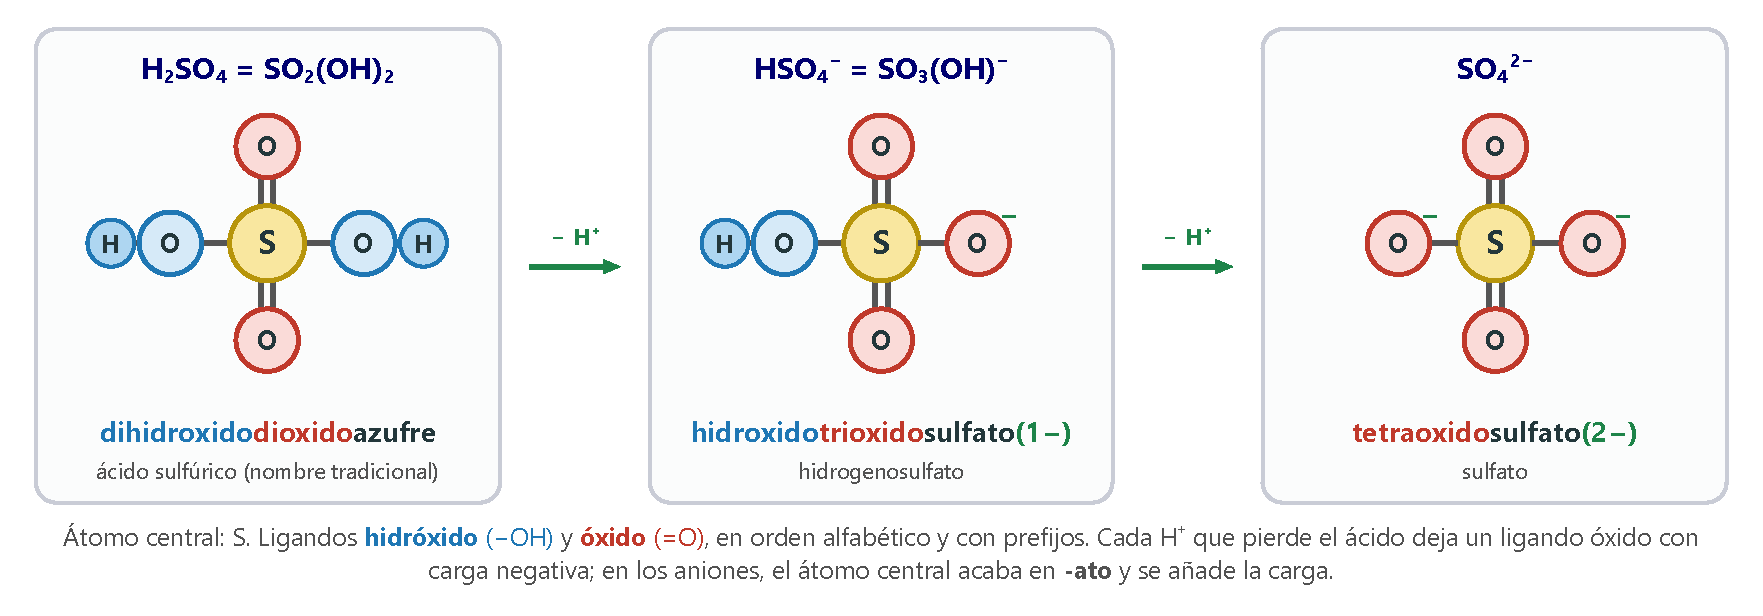
\includegraphics[width=\textwidth]{images/UD5/adicion_oxoacido}
    \caption{Nomenclatura de adición del ácido sulfúrico y de los aniones que se forman cuando pierde sus iones \ch{H+}.}
    \label{fig:ud5-adicion}
\end{figure}

\begin{table}[H]
    \centering
    \caption{Nombres de algunos oxoácidos en los tres sistemas}
    \vspace{-5pt}
    \small
    \setlength{\tabcolsep}{5pt}
    \begin{tabular}{@{}llL{4.35cm}L{4.1cm}@{}}
        \toprule
        \textbf{Fórmula} & \textbf{Tradicional} & \textbf{Hidrógeno} & \textbf{Adición} \\
        \midrule
        \ch{H3BO3} \(=\) \ch{B(OH)3} & ácido bórico & trihidrogeno(trioxidoborato) & trihidroxidoboro \\[3pt]
        \ch{H2CO3} \(=\) \ch{CO(OH)2} & ácido carbónico & dihidrogeno(trioxidocarbonato) & dihidroxidooxidocarbono \\[3pt]
        \ch{HNO2} \(=\) \ch{NO(OH)} & ácido nitroso & hidrogeno(dioxidonitrato) & hidroxidooxidonitrógeno \\[3pt]
        \ch{H3PO4} \(=\) \ch{PO(OH)3} & ácido fosfórico & trihidrogeno(tetraoxidofosfato) & trihidroxidooxidofósforo \\[3pt]
        \ch{H2SO4} \(=\) \ch{SO2(OH)2} & ácido sulfúrico & dihidrogeno(tetraoxidosulfato) & dihidroxidodioxidoazufre \\[3pt]
        \ch{HClO} \(=\) \ch{Cl(OH)} & ácido hipocloroso & hidrogeno(oxidoclorato) & hidroxidocloro \\[3pt]
        \ch{HIO3} \(=\) \ch{IO2(OH)} & ácido yódico & hidrogeno(trioxidoyodato) & hidroxidodioxidoyodo \\
        \bottomrule
    \end{tabular}
    \label{tab:ud5-oxoacidos-nombres}
\end{table}

\begin{example}
    \textbf{Oxoácidos.} a) Nombra el \ch{HBrO2} y el \ch{H4SiO4} en los tres sistemas. b) Formula el
    hidrogeno(tetraoxidomanganato) y el dihidroxidodioxidoselenio.

    \textbf{Solución.} a) \ch{HBrO2}: en la nomenclatura de hidrógeno, 1 H, 2 O y 1 Br: hidrogeno(dioxidobromato). Para la de
    adición se reescribe como \ch{BrO(OH)}: hidroxidooxidobromo. El estado de oxidación del Br es \(1 + x - 4 = 0\), \(x = +3\),
    el segundo de sus cuatro estados positivos: ácido \textbf{bromoso}.

    \ch{H4SiO4}: tetrahidrogeno(tetraoxidosilicato); \ch{Si(OH)4}, tetrahidroxidosilicio; ácido silícico.

    b) Hidrogeno(tetraoxidomanganato): 1 H, 4 O y 1 Mn: \ch{HMnO4} (ácido permangánico). Dihidroxidodioxidoselenio:
    \ch{SeO2(OH)2}, es decir, 2 H, 1 Se y 4 O: \ch{H2SeO4} (ácido selénico).
\end{example}

\begin{exercise}
    Nombra con la nomenclatura de hidrógeno y con la de adición, y da el nombre tradicional: a) \ch{HNO3}; b) \ch{H2SO3}; c)
    \ch{HClO4}; d) \ch{H3AsO4}; e) \ch{HIO}; f) \ch{H2TeO4}; g) \ch{HBrO3}; h) \ch{H3PO3}.
    \begin{solu}
        a) \textcolor{red}{hidrogeno(trioxidonitrato); \ch{NO2(OH)}, hidroxidodioxidonitrógeno; ácido nítrico}.
        b) \textcolor{red}{dihidrogeno(trioxidosulfato); \ch{SO(OH)2}, dihidroxidooxidoazufre; ácido sulfuroso}.
        c) \textcolor{red}{hidrogeno(tetraoxidoclorato); \ch{ClO3(OH)}, hidroxidotrioxidocloro; ácido perclórico}.
        d) \textcolor{red}{trihidrogeno(tetraoxidoarseniato); \ch{AsO(OH)3}, trihidroxidooxidoarsénico; ácido arsénico}.
        e) \textcolor{red}{hidrogeno(oxidoyodato); \ch{I(OH)}, hidroxidoyodo; ácido hipoyodoso}.
        f) \textcolor{red}{dihidrogeno(tetraoxidotelurato); \ch{TeO2(OH)2}, dihidroxidodioxidoteluro; ácido telúrico}.
        g) \textcolor{red}{hidrogeno(trioxidobromato); \ch{BrO2(OH)}, hidroxidodioxidobromo; ácido brómico}.
        h) \textcolor{red}{trihidrogeno(trioxidofosfato); \ch{P(OH)3}, trihidroxidofósforo; ácido fosforoso}.
    \end{solu}
\end{exercise}

\begin{exercise}
    Formula: a) hidrogeno(dioxidoclorato); b) dihidrogeno(trioxidocarbonato); c) trihidrogeno(tetraoxidofosfato); d)
    dihidrogeno(tetraoxidocromato); e) hidroxidodioxidocloro; f) tetrahidroxidosilicio; g) dihidroxidooxidoselenio; h)
    hidroxidotrioxidoyodo; i) ácido nitroso; j) ácido disulfúrico.
    \begin{solu}
        a) \textcolor{red}{\ch{HClO2}}; b) \textcolor{red}{\ch{H2CO3}}; c) \textcolor{red}{\ch{H3PO4}}; d)
        \textcolor{red}{\ch{H2CrO4}}; e) \textcolor{red}{\ch{HClO3}}; f) \textcolor{red}{\ch{H4SiO4}}; g)
        \textcolor{red}{\ch{H2SeO3}}; h) \textcolor{red}{\ch{HIO4}}; i) \textcolor{red}{\ch{HNO2}}; j)
        \textcolor{red}{\ch{H2S2O7}}.
    \end{solu}
\end{exercise}

\subsection{Oxoaniones}\label{sec:ud5-oxoaniones}

\begin{definition}[Oxoanión]
    Es el anión que queda cuando un oxoácido \textbf{pierde} uno o varios \textbf{iones \ch{H+}}. Tiene tantas \textbf{cargas
    negativas} como iones \ch{H+} ha perdido.
\end{definition}

El ácido carbónico, \ch{H2CO3}, puede perder sus dos \ch{H+} y dar el ion \ch{CO3^2-}, o perder solo uno y dar el
\ch{HCO3-}. Los oxoaniones que conservan algún hidrógeno se llaman \textbf{oxoaniones ácidos}.

\paragraph{Nombres tradicionales.} La IUPAC los admite para los oxoaniones que proceden de los ácidos de la
tabla~\ref{tab:ud5-oxoacidos}. Se cambia la terminación del ácido: \textbf{-oso} pasa a \textbf{-ito} e \textbf{-ico} pasa a
\textbf{-ato}, y se quita la palabra «ácido». Si quedan hidrógenos, se indica cuántos con el prefijo \textbf{hidrogeno}:
\begin{itemize}
    \item \ch{ClO-}, del ácido hipocloroso: \textbf{hipoclorito}. \ch{NO3-}, del ácido nítrico: \textbf{nitrato}.
    \ch{S2O7^2-}, del ácido disulfúrico: \textbf{disulfato}.
    \item \ch{H2PO4-}, del ácido fosfórico, que ha perdido un \ch{H+} y conserva dos: \textbf{dihidrogenofosfato}.
    \item Conviene conocer también \ch{CrO4^2-}, \textbf{cromato}; \ch{Cr2O7^2-}, \textbf{dicromato}; \ch{MnO4^2-},
    \textbf{manganato}, y \ch{MnO4-}, \textbf{permanganato}.
\end{itemize}

\paragraph{Nomenclatura de composición.} Se nombran los oxígenos con su prefijo, «oxido», la raíz del elemento central
terminada en \textbf{-ato} y el número de carga: \ch{SO4^2-} es el \textbf{tetraoxidosulfato(2\nobreakdash--)} y \ch{Cr2O7^2-}, el
\textbf{heptaoxidodicromato(2\nobreakdash--)}. Formular es inmediato a partir del nombre.

\paragraph{Nomenclatura de hidrógeno.} Solo se usa en los \textbf{oxoaniones ácidos}: se antepone el prefijo hidrogeno al nombre
de composición entre paréntesis y se añade la carga: \ch{H2PO4-} es el \textbf{dihidrogeno(tetraoxidofosfato)(1\nobreakdash--)}.

\paragraph{Nomenclatura de adición.} Se construye como en los oxoácidos, pero el átomo central termina en \textbf{-ato} y se
añade el número de carga: \ch{HSO3-} \(=\) \ch{SO2(OH)-} es el \textbf{hidroxidodioxidosulfato(1\nobreakdash--)}. Si el oxoanión no tiene
hidrógeno, el nombre coincide con el de composición (figura~\ref{fig:ud5-adicion}).

\begin{table}[H]
    \centering
    \caption{Nombres de algunos oxoaniones}
    \vspace{-5pt}
    \small
    \begin{tabular}{@{}lL{3.0cm}L{4.9cm}L{4.5cm}@{}}
        \toprule
        \textbf{Fórmula} & \textbf{Tradicional} & \textbf{Composición o hidrógeno} & \textbf{Adición} \\
        \midrule
        \ch{NO2-} & nitrito & dioxidonitrato(1\nobreakdash--) & dioxidonitrato(1\nobreakdash--) \\[3pt]
        \ch{CO3^2-} & carbonato & trioxidocarbonato(2\nobreakdash--) & trioxidocarbonato(2\nobreakdash--) \\[3pt]
        \ch{PO4^3-} & fosfato & tetraoxidofosfato(3\nobreakdash--) & tetraoxidofosfato(3\nobreakdash--) \\[3pt]
        \ch{ClO3-} & clorato & trioxidoclorato(1\nobreakdash--) & trioxidoclorato(1\nobreakdash--) \\[3pt]
        \ch{HCO3-} & hidrogenocarbonato & hidrogeno(trioxidocarbonato)(1\nobreakdash--) & hidroxidodioxidocarbonato(1\nobreakdash--) \\[3pt]
        \ch{HPO4^2-} & hidrogenofosfato & hidrogeno(tetraoxidofosfato)(2\nobreakdash--) & hidroxidotrioxidofosfato(2\nobreakdash--) \\[3pt]
        \ch{H2PO4-} & dihidrogenofosfato & dihidrogeno(tetraoxidofosfato)(1\nobreakdash--) & dihidroxidodioxidofosfato(1\nobreakdash--) \\[3pt]
        \ch{HSO4-} & hidrogenosulfato & hidrogeno(tetraoxidosulfato)(1\nobreakdash--) & hidroxidotrioxidosulfato(1\nobreakdash--) \\
        \bottomrule
    \end{tabular}
    \label{tab:ud5-oxoaniones}
\end{table}

\begin{example}
    \textbf{Oxoaniones.} a) ¿Qué oxoaniones puede formar el ácido sulfuroso? Nómbralos. b) Formula el ion
    trioxidoarseniato(3\nobreakdash--) y el hidroxidotrioxidofosfato(2\nobreakdash--).

    \textbf{Solución.} a) El \ch{H2SO3} puede perder un \ch{H+}: \ch{HSO3-}, hidrogenosulfito; hidrogeno(trioxidosulfato)(1\nobreakdash--);
    \ch{SO2(OH)-}, hidroxidodioxidosulfato(1\nobreakdash--). O los dos: \ch{SO3^2-}, sulfito; trioxidosulfato(2\nobreakdash--).

    b) Trioxidoarseniato(3\nobreakdash--): 3 O y 1 As con carga \(-3\): \ch{AsO3^3-} (arsenito, del ácido arsenoso).
    Hidroxidotrioxidofosfato(2\nobreakdash--): un ligando \ch{OH} y tres óxido unidos a un fósforo, \ch{PO3(OH)^2-}; reagrupando,
    \ch{HPO4^2-} (hidrogenofosfato). Comprobamos el estado de oxidación del P: \(1 + x - 8 = -2\), \(x = +5\), el mismo que en
    el ácido fosfórico.
\end{example}

\begin{exercise}
    Nombra con la nomenclatura de composición (o de hidrógeno, si tienen H) y da el nombre tradicional: a) \ch{SO3^2-}; b)
    \ch{BrO-}; c) \ch{IO4-}; d) \ch{SiO4^4-}; e) \ch{SeO4^2-}; f) \ch{BO3^3-}; g) \ch{HSeO4-}; h) \ch{H2AsO4-}; i) \ch{HCO3-};
    j) \ch{HPO4^2-}.
    \begin{solu}
        a) \textcolor{red}{trioxidosulfato(2\nobreakdash--); sulfito}. b) \textcolor{red}{oxidobromato(1\nobreakdash--); hipobromito}. c)
        \textcolor{red}{tetraoxidoyodato(1\nobreakdash--); peryodato}. d) \textcolor{red}{tetraoxidosilicato(4\nobreakdash--); silicato}. e)
        \textcolor{red}{tetraoxidoseleniato(2\nobreakdash--); seleniato}. f) \textcolor{red}{trioxidoborato(3\nobreakdash--); borato}. g)
        \textcolor{red}{hidrogeno(tetraoxidoseleniato)(1\nobreakdash--); hidrogenoseleniato}. h)
        \textcolor{red}{dihidrogeno(tetraoxidoarseniato)(1\nobreakdash--); dihidrogenoarseniato}. i)
        \textcolor{red}{hidrogeno(trioxidocarbonato)(1\nobreakdash--); hidrogenocarbonato}. j)
        \textcolor{red}{hidrogeno(tetraoxidofosfato)(2\nobreakdash--); hidrogenofosfato}.
    \end{solu}
\end{exercise}

\begin{exercise}
    a) Nombra con la nomenclatura de adición: \ch{HSO4-}, \ch{H2PO4-}, \ch{HCO3-}, \ch{HSeO3-}. b) Formula: trioxidonitrato(1\nobreakdash--),
    tetraoxidomanganato(1\nobreakdash--), dioxidoclorato(1\nobreakdash--), heptaoxidodicromato(2\nobreakdash--), hidrogeno(trioxidosulfato)(1\nobreakdash--), perclorato,
    cromato, hidroxidodioxidoarseniato(2\nobreakdash--).
    \begin{solu}
        a) \ch{SO3(OH)-}: \textcolor{red}{hidroxidotrioxidosulfato(1\nobreakdash--)}; \ch{PO2(OH)2-}: \textcolor{red}{dihidroxidodioxidofosfato(1\nobreakdash--)};
        \ch{CO2(OH)-}: \textcolor{red}{hidroxidodioxidocarbonato(1\nobreakdash--)}; \ch{SeO2(OH)-}:
        \textcolor{red}{hidroxidodioxidoseleniato(1\nobreakdash--)}. b) \textcolor{red}{\ch{NO3-}, \ch{MnO4-}, \ch{ClO2-}, \ch{Cr2O7^2-},
        \ch{HSO3-}, \ch{ClO4-}, \ch{CrO4^2-}}, \ch{AsO2(OH)^2-} \(=\) \textcolor{red}{\ch{HAsO3^2-}}.
    \end{solu}
\end{exercise}

\subsection{Oxosales}\label{sec:ud5-oxosales}

\begin{definition}[Oxosal]
    Es un compuesto formado por un \textbf{catión} y un \textbf{oxoanión}, combinados en la proporción necesaria para que el
    compuesto sea \textbf{neutro}.
\end{definition}

Para formular, se escribe el catión seguido del anión, con los números de cada uno como subíndices; el anión (y el catión, si es
poliatómico) va entre paréntesis si su subíndice es mayor que 1. Se nombra primero el anión y después el catión, como en un
compuesto binario. Para manejar las oxosales es imprescindible dominar antes los oxoaniones.

\paragraph{Nombre tradicional.} Se nombra el anión con su nombre tradicional y el catión con su número de oxidación (o de
carga) si tiene más de uno: sulfato de hierro(III).
\begin{itemize}
    \item \textbf{Formular}: sulfato de hierro(III). El anión es \ch{SO4^2-} y el catión, \ch{Fe^3+}. El mínimo común múltiplo
    de las cargas (2 y 3) es 6: hacen falta \textbf{3 aniones} y \textbf{2 cationes}: \ch{Fe2(SO4)3}.
    \item \textbf{Nombrar}: se separan catión y anión y se averigua la carga de cada uno. En el \ch{Fe2(SO4)3} hay 2 cationes y
    3 aniones; como las cargas totales tienen que ser iguales (6), cada anión tiene carga \(-2\) y cada catión, \(+3\).
\end{itemize}

No siempre es tan inmediato. En el \ch{CuBrO3}, el catión podría ser \ch{Cu+} o \ch{Cu^2+}. Si fuera \ch{Cu^2+}, el anión
sería \ch{BrO3^2-} y el bromo tendría \(x - 6 = -2\), \(x = +4\), que no es un estado de oxidación del bromo. Con \ch{Cu+} el
anión es \ch{BrO3-} (\(x = +5\), correcto): la sal es el \textbf{bromato de cobre(I)}.

\paragraph{Nomenclatura de composición.} La proporción se indica con prefijos multiplicadores; para el anión, que ya lleva
prefijos, se usan los \textbf{complejos} (bis, tris…) y su nombre va entre paréntesis: \ch{Ca(PO3)2} es el
bis(trioxidofosfato) de calcio, y el tris(tetraoxidosulfato) de dioro es \ch{Au2(SO4)3}.

\paragraph{Nomenclatura de adición.} Se nombran el anión y el catión con sus números de carga, sin indicar la proporción: el
\ch{K2Cr2O7} es el heptaoxidodicromato(2\nobreakdash--) de potasio. Para formular hay que calcular los subíndices, sabiendo que el compuesto
es neutro (dos \ch{K+} por cada \ch{Cr2O7^2-}). Para nombrar, primero hay que averiguar las cargas: en el \ch{FeSO4}, si el
catión fuera \ch{Fe^3+}, el anión sería \ch{SO4^3-} y el azufre tendría \(+5\), que no es válido; el catión es \ch{Fe^2+} y la
sal es el tetraoxidosulfato(2\nobreakdash--) de hierro(2+).

\begin{table}[H]
    \centering
    \caption{Nombres de algunas oxosales}
    \vspace{-5pt}
    \small
    \begin{tabular}{@{}lL{3.2cm}L{4.2cm}L{4.6cm}@{}}
        \toprule
        \textbf{Fórmula} & \textbf{Tradicional} & \textbf{Composición} & \textbf{Adición} \\
        \midrule
        \ch{NaClO} & hipoclorito de sodio & oxidoclorato de sodio & oxidoclorato(1\nobreakdash--) de sodio \\[3pt]
        \ch{CaCO3} & carbonato de calcio & trioxidocarbonato de calcio & trioxidocarbonato(2\nobreakdash--) de calcio \\[3pt]
        \ch{Fe2(SO4)3} & sulfato de hierro(III) & tris(tetraoxidosulfato) de dihierro & tetraoxidosulfato(2\nobreakdash--) de hierro(3+) \\[3pt]
        \ch{Ca3(PO4)2} & fosfato de calcio & bis(tetraoxidofosfato) de tricalcio & tetraoxidofosfato(3\nobreakdash--) de calcio \\[3pt]
        \ch{Pb(NO3)4} & nitrato de plomo(IV) & tetrakis(trioxidonitrato) de plomo & trioxidonitrato(1\nobreakdash--) de plomo(4+) \\[3pt]
        \ch{KMnO4} & permanganato de potasio & tetraoxidomanganato de potasio & tetraoxidomanganato(1\nobreakdash--) de potasio \\
        \bottomrule
    \end{tabular}
    \label{tab:ud5-oxosales}
\end{table}

\begin{example}
    \textbf{Oxosales.} a) Nombra el \ch{Pb(CO3)2} en los tres sistemas. b) Formula el clorito de aluminio y el
    bis(tetraoxidoclorato) de cobre.

    \textbf{Solución.} a) Hay 2 aniones \ch{CO3}. Si el catión fuera \ch{Pb^2+}, cada anión sería \ch{CO3-} y el carbono tendría
    \(x - 6 = -1\), \(x = +5\): imposible. El anión es \ch{CO3^2-} (carbonato) y el catión, \ch{Pb^4+}. Nombres: carbonato de
    plomo(IV); bis(trioxidocarbonato) de plomo; trioxidocarbonato(2\nobreakdash--) de plomo(4+).

    b) Clorito: \ch{ClO2-} (del ácido cloroso); aluminio: \ch{Al^3+}. Hacen falta 3 aniones por cada catión: \ch{Al(ClO2)3}.
    Bis(tetraoxidoclorato) de cobre: dos aniones \ch{ClO4-} y un cobre: \ch{Cu(ClO4)2}.
\end{example}

\begin{exercise}
    Determina las cargas del catión y del anión y da el nombre tradicional de: a) \ch{NaNO2}; b) \ch{Fe(NO3)3}; c) \ch{Hg2SO4};
    d) \ch{K2CrO4}; e) \ch{Al2(SO3)3}; f) \ch{Mg3(PO4)2}; g) \ch{Cu(IO3)2}; h) \ch{Ba(MnO4)2}.
    \begin{solu}
        a) \ch{Na+} y \ch{NO2-}: \textcolor{red}{nitrito de sodio}. b) \ch{Fe^3+} y \ch{NO3-}: \textcolor{red}{nitrato de
        hierro(III)}. c) \ch{Hg2^2+} (o \ch{Hg+}) y \ch{SO4^2-}: \textcolor{red}{sulfato de mercurio(I)}. d) \ch{K+} y \ch{CrO4^2-}:
        \textcolor{red}{cromato de potasio}. e) \ch{Al^3+} y \ch{SO3^2-}: \textcolor{red}{sulfito de aluminio}. f) \ch{Mg^2+} y
        \ch{PO4^3-}: \textcolor{red}{fosfato de magnesio}. g) \ch{Cu^2+} y \ch{IO3-}: \textcolor{red}{yodato de cobre(II)}.
        h) \ch{Ba^2+} y \ch{MnO4-}: \textcolor{red}{permanganato de bario}.
    \end{solu}
\end{exercise}

\begin{exercise}
    a) Nombra con la nomenclatura de composición y con la de adición: \ch{Na2SO4}, \ch{Ni(ClO3)2}, \ch{Al(NO3)3},
    \ch{Co2(CO3)3}. b) Formula: carbonato de sodio, nitrato de plata, perclorato de potasio, sulfato de cobre(II), fosfato de
    hierro(II), bis(trioxidonitrato) de calcio, tris(tetraoxidosulfato) de dicromo, tetraoxidomanganato(1\nobreakdash--) de sodio,
    trioxidoyodato(1\nobreakdash--) de plomo(2+).
    \begin{solu}
        a) \textcolor{red}{tetraoxidosulfato de disodio; tetraoxidosulfato(2\nobreakdash--) de sodio}. \textcolor{red}{bis(trioxidoclorato) de
        níquel; trioxidoclorato(1\nobreakdash--) de níquel(2+)}. \textcolor{red}{tris(trioxidonitrato) de aluminio; trioxidonitrato(1\nobreakdash--) de
        aluminio}. \textcolor{red}{tris(trioxidocarbonato) de dicobalto; trioxidocarbonato(2\nobreakdash--) de cobalto(3+)}.
        b) \textcolor{red}{\ch{Na2CO3}, \ch{AgNO3}, \ch{KClO4}, \ch{CuSO4}, \ch{Fe3(PO4)2}, \ch{Ca(NO3)2}, \ch{Cr2(SO4)3},
        \ch{NaMnO4}, \ch{Pb(IO3)2}}.
    \end{solu}
\end{exercise}

\subsection{Sales ácidas}\label{sec:ud5-sales-acidas}

\paragraph{Sales ácidas de oxoácidos.} Están formadas por un catión y un \textbf{oxoanión ácido}, que procede de un oxoácido que
no ha perdido todos sus hidrógenos. Todo lo dicho para las oxosales es válido; solo hay que saber nombrar y formular el anión.

\paragraph{Sales ácidas de haluros de hidrógeno.} Las disoluciones de \ch{H2S}, \ch{H2Se} y \ch{H2Te} son ácidas. Si pierden solo
uno de sus dos \ch{H+}, quedan los aniones \ch{HS-}, \ch{HSe-} y \ch{HTe-}, que forman sales con los cationes: \ch{KHS} es el
hidrogenosulfuro de potasio o hidrogeno(sulfuro) de potasio. Los haluros del grupo 17 (\ch{HCl}…) solo tienen un hidrógeno y no
forman sales ácidas.

\begin{table}[H]
    \centering
    \caption{Nombres de algunas sales ácidas}
    \vspace{-5pt}
    \begin{tabular}{@{}lllL{3.6cm}L{5.4cm}@{}}
        \toprule
        \textbf{Fórmula} & \textbf{Catión} & \textbf{Anión} & \textbf{Tradicional} & \textbf{Composición} \\
        \midrule
        \ch{NaHSO4} & \ch{Na+} & \ch{HSO4-} & hidrogenosulfato de sodio & hidrogeno(tetraoxidosulfato) de sodio \\[3pt]
        \ch{Ca(HCO3)2} & \ch{Ca^2+} & \ch{HCO3-} & hidrogenocarbonato de calcio & bis[hidrogeno(trioxidocarbonato)] de calcio \\[3pt]
        \ch{KH2PO4} & \ch{K+} & \ch{H2PO4-} & dihidrogenofosfato de potasio & dihidrogeno(tetraoxidofosfato) de potasio \\[3pt]
        \ch{Fe(HS)2} & \ch{Fe^2+} & \ch{HS-} & hidrogenosulfuro de hierro(II) & bis[hidrogeno(sulfuro)] de hierro \\[3pt]
        \ch{NH4HSe} & \ch{NH4+} & \ch{HSe-} & hidrogenoseleniuro de amonio & hidrogeno(seleniuro) de amonio \\
        \bottomrule
    \end{tabular}
    \label{tab:ud5-sales-acidas}
\end{table}

Fíjate en que, cuando el nombre del anión ya lleva paréntesis y hay que multiplicarlo, se usan \textbf{corchetes}:
bis[hidrogeno(trioxidocarbonato)]. El hidrogenocarbonato de sodio, \ch{NaHCO3}, es el «bicarbonato» de la cocina; el
nombre bicarbonato no es aceptado por la IUPAC.

\begin{exercise}
    a) Nombra: \ch{KHCO3}, \ch{Mg(HSO4)2}, \ch{Na2HPO4}, \ch{LiH2PO4}, \ch{Ba(HS)2}, \ch{CuHSO3}, \ch{NaHSe}, \ch{Fe(HCO3)3}. b)
    Formula: hidrogenocarbonato de magnesio, hidrogenosulfato de potasio, dihidrogenofosfato de calcio, hidrogenosulfuro de
    sodio, hidrogeno(tetraoxidosulfato) de plata, hidrogenosulfito de aluminio, hidrogenotelururo de cobre(II).
    \begin{solu}
        a) \textcolor{red}{hidrogenocarbonato de potasio}; \textcolor{red}{hidrogenosulfato de magnesio}; \textcolor{red}{hidrogenofosfato
        de sodio}; \textcolor{red}{dihidrogenofosfato de litio}; \textcolor{red}{hidrogenosulfuro de bario};
        \textcolor{red}{hidrogenosulfito de cobre(I)}; \textcolor{red}{hidrogenoseleniuro de sodio};
        \textcolor{red}{hidrogenocarbonato de hierro(III)}. b) \textcolor{red}{\ch{Mg(HCO3)2}, \ch{KHSO4}, \ch{Ca(H2PO4)2},
        \ch{NaHS}, \ch{AgHSO4}, \ch{Al(HSO3)3}, \ch{Cu(HTe)2}}.
    \end{solu}
\end{exercise}

\subsection{Sales hidratadas}\label{sec:ud5-hidratadas}

\begin{definition}[Sal hidratada]
    Es una sal que contiene moléculas de \textbf{agua} en su estructura cristalina, en una proporción fija. En la fórmula, las
    moléculas de agua se escriben detrás de un punto centrado: \ch{CuSO4 * 5 H2O}.
\end{definition}

Se nombra la sal por cualquiera de los sistemas válidos, seguida de «agua» y, entre paréntesis, la proporción sal/agua; o bien
se añade la palabra hidrato con el prefijo multiplicador correspondiente:
\begin{itemize}
    \item \ch{Na2CO3 * 10 H2O}: carbonato de sodio---agua (1/10) o carbonato de sodio decahidrato.
    \item \ch{FeCl3 * 6 H2O}: tricloruro de hierro---agua (1/6) o tricloruro de hierro hexahidrato.
    \item \ch{3 CdSO4 * 8 H2O}: sulfato de cadmio---agua (3/8). Aquí solo sirve la primera forma, porque la proporción no es un
    número entero de moléculas de agua por cada unidad de sal.
\end{itemize}
Al calentarlas, estas sales pierden el agua: el sulfato de cobre(II) pentahidrato, azul, se vuelve blanco al deshidratarse
(práctica de la sección~\ref{sec:ud5-practicas}).

\begin{exercise}
    a) Nombra: \ch{MgSO4 * 7 H2O}, \ch{CaCl2 * 2 H2O}, \ch{CoCl2 * 6 H2O}, \ch{Na2SO4 * 10 H2O}. b) Formula: sulfato de calcio
    dihidrato, cloruro de bario---agua (1/2), nitrato de níquel(II) hexahidrato, carbonato de sodio---agua (1/1).
    \begin{solu}
        a) \textcolor{red}{sulfato de magnesio heptahidrato} (sulfato de magnesio---agua (1/7)); \textcolor{red}{cloruro de
        calcio dihidrato}; \textcolor{red}{cloruro de cobalto(II) hexahidrato}; \textcolor{red}{sulfato de sodio decahidrato}.
        b) \textcolor{red}{\ch{CaSO4 * 2 H2O}, \ch{BaCl2 * 2 H2O}, \ch{Ni(NO3)2 * 6 H2O}, \ch{Na2CO3 * H2O}}.
    \end{solu}
\end{exercise}

\begin{exercise}
    El yeso es sulfato de calcio dihidrato. a) Escribe su fórmula. b) ¿Qué porcentaje de su masa es agua?
    (\(M(\ch{Ca}) = 40{,}1\), \(M(\ch{S}) = 32{,}1\), \(M(\ch{O}) = 16{,}0\), \(M(\ch{H}) = 1{,}0\) en \unit{\gram\per\mol}).
    \begin{solu}
        a) \textcolor{red}{\ch{CaSO4 * 2 H2O}}. b) \(M(\ch{CaSO4}) = 40{,}1 + 32{,}1 + 64{,}0 = \qty{136.2}{\gram\per\mol}\);
        \(M(2\,\ch{H2O}) = \qty{36.0}{\gram\per\mol}\); \(M = \qty{172.2}{\gram\per\mol}\).
        \(\dfrac{36{,}0}{172{,}2} \cdot 100 = \textcolor{red}{\qty{20.9}{\percent}}\).
    \end{solu}
\end{exercise}

%========================================================================================
\section{Química en la vida: de la alquimia a la IUPAC}\label{sec:ud5-historia}
%========================================================================================

Hasta finales del siglo \textsc{xviii}, cada sustancia tenía un nombre heredado de la alquimia, del comercio o de la farmacia:
aceite de vitriolo (ácido sulfúrico), espíritu de sal (ácido clorhídrico), sal de Glauber (sulfato de sodio decahidrato), flores
de cinc (óxido de cinc)\dots{} Un mismo compuesto podía tener varios nombres y un mismo nombre servir para sustancias distintas.

En 1787, cuatro químicos franceses, \textbf{Guyton de Morveau}, \textbf{Lavoisier}, \textbf{Berthollet} y \textbf{Fourcroy},
publicaron el \textit{Método de nomenclatura química}. Su idea era revolucionaria: el nombre de un compuesto debía indicar
\textbf{de qué está hecho}. De ahí vienen los óxidos, los sulfatos o los nitratos, y las terminaciones -oso e -ico para
distinguir la «cantidad de oxígeno». Poco después, \textbf{Berzelius} propuso escribir los elementos con una o dos letras de su
nombre latino, que es el origen de nuestros símbolos (Na de \textit{natrium}, Fe de \textit{ferrum}, S de \textit{sulphur}).

El número de compuestos conocidos no dejó de crecer, y en el siglo \textsc{xx} se hizo necesario un organismo internacional que
pusiera orden: la IUPAC, fundada en 1919, publica periódicamente sus recomendaciones, conocidas por el color de las tapas. El
\textbf{Libro Rojo} recoge la nomenclatura inorgánica; su versión vigente es de 2005. Muchos nombres que aprendieron tus padres
(anhídridos, ácido sulfhídrico, bicarbonato) ya no se recomiendan, y otros nuevos, como dihidrogeno(tetraoxidosulfato), se
basan en la estructura de las moléculas. La química sigue cambiando, y su lenguaje también.

\begin{exercise}
    a) ¿Qué principio introdujo el \textit{Método de nomenclatura química} de 1787? b) La sal de Glauber es sulfato de sodio
    decahidrato y el aceite de vitriolo, ácido sulfúrico. Escribe sus fórmulas. c) ¿Por qué el nombre «bicarbonato» no indica
    bien la composición del \ch{NaHCO3}?
    \begin{solu}
        a) \textcolor{red}{Que el nombre de un compuesto indique de qué elementos está formado.} b) \textcolor{red}{\ch{Na2SO4 *
        10 H2O} y \ch{H2SO4}}. c) \textcolor{red}{El prefijo bi- sugiere que hay dos carbonatos}, cuando en realidad la sal tiene
        un anión carbonato con un hidrógeno (\ch{HCO3-}); el nombre correcto es hidrogenocarbonato de sodio.
    \end{solu}
\end{exercise}

%========================================================================================
\section{Prácticas}\label{sec:ud5-practicas}
%========================================================================================

\subsection{Química en casa: la química de las etiquetas}

\noindent\begin{minipage}[t]{0.48\textwidth}
    \textbf{Objetivo}
    \begin{itemize}
        \item Identificar compuestos inorgánicos en las etiquetas de productos cotidianos, escribir su fórmula y nombrarlos
        correctamente.
    \end{itemize}
\end{minipage}\hfill
\begin{minipage}[t]{0.48\textwidth}
    \textbf{Material}
    \begin{itemize}
        \item Envases o fotografías de las etiquetas de productos de limpieza, de higiene, de alimentación y de jardinería:
        lejía, salfumán, pasta de dientes, sal yodada, bicarbonato, agua mineral, abono, productos para piscinas\dots
    \end{itemize}
\end{minipage}

\textbf{Procedimiento}
\begin{enumerate}[label=\numberballgreen]
    \item Busca en cada etiqueta la composición o los ingredientes y anota los compuestos inorgánicos que aparezcan.
    \item Para cada uno, escribe su fórmula, el tipo de compuesto y su nombre en al menos dos sistemas de nomenclatura.
    \item Señala los nombres de las etiquetas que no siguen las normas de la IUPAC y corrígelos.
    \item Anota los pictogramas de peligro de cada producto y las advertencias de uso.
\end{enumerate}
\textbf{No abras ni mezcles los productos: trabaja solo con las etiquetas.}

\begin{exercise}
    Algunos compuestos que suelen aparecer en las etiquetas son: hipoclorito de sodio (lejía), fluoruro de sodio (pasta de
    dientes), yoduro de potasio (sal yodada), «bicarbonato sódico», «cloruro magnésico» y «sulfato cálcico» (aguas minerales) y
    nitrato de amonio (abonos). a) Escribe sus fórmulas. b) Corrige los nombres que no siguen las normas de la IUPAC. c) ¿Qué tipo
    de compuesto es cada uno?
    \begin{solu}
        a) \textcolor{red}{\ch{NaClO}, \ch{NaF}, \ch{KI}, \ch{NaHCO3}, \ch{MgCl2}, \ch{CaSO4}, \ch{NH4NO3}}. b)
        \textcolor{red}{Hidrogenocarbonato de sodio, cloruro de magnesio y sulfato de calcio} (no se usan los adjetivos
        «sódico», «magnésico», «cálcico»). c) \textcolor{red}{\ch{NaF}, \ch{KI} y \ch{MgCl2}: sales binarias; \ch{NaClO},
        \ch{CaSO4} y \ch{NH4NO3}: oxosales; \ch{NaHCO3}: sal ácida.}
    \end{solu}
\end{exercise}

\subsection{¿Cuánta agua tiene una sal hidratada?}

\noindent\begin{minipage}[t]{0.48\textwidth}
    \textbf{Objetivo}
    \begin{itemize}
        \item Determinar experimentalmente el número de moléculas de agua de hidratación del sulfato de cobre(II).
    \end{itemize}
\end{minipage}\hfill
\begin{minipage}[t]{0.48\textwidth}
    \textbf{Material y reactivos}
    \begin{itemize}
        \item Crisol de porcelana (o cápsula), triángulo de arcilla, trípode, mechero, pinzas, desecador y balanza de
        precisión (\qty{0.01}{\gram}).
        \item Sulfato de cobre(II) hidratado (cristales azules) y unas gotas de agua.
    \end{itemize}
\end{minipage}

\textbf{Procedimiento}
\begin{enumerate}[label=\numberballgreen]
    \item Pesa el crisol limpio y seco (\(m_1\)). Añade unos \qty{2}{\gram} de sulfato de cobre hidratado, triturado, y pesa
    de nuevo (\(m_2\)).
    \item Calienta suavemente, removiendo con una varilla, hasta que todo el sólido pase de azul a blanco grisáceo. Evita
    calentar al rojo: el sulfato se descompondría.
    \item Deja enfriar el crisol en el desecador y pésalo (\(m_3\)). Calienta otra vez unos minutos y vuelve a pesar, hasta que
    la masa no cambie.
    \item Deja caer unas gotas de agua sobre el sólido blanco y observa qué ocurre.
\end{enumerate}
\textbf{Usa gafas y pinzas: el crisol quema. El sulfato de cobre es nocivo: lávate las manos al terminar.}

\begin{exercise}
    En una práctica se obtuvieron \(m_1 = \qty{24.36}{\gram}\), \(m_2 = \qty{26.41}{\gram}\) y \(m_3 = \qty{25.67}{\gram}\).
    a) Calcula la masa de sal anhidra y la de agua perdida. b) Calcula los moles de cada una y la fórmula de la sal hidratada
    (\(M(\ch{CuSO4}) = \qty{159.6}{\gram\per\mol}\)). c) Nombra la sal. d) ¿Qué ocurre al añadir agua al sólido blanco?
    \begin{solu}
        a) \(m(\ch{CuSO4}) = 25{,}67 - 24{,}36 = \textcolor{red}{\qty{1.31}{\gram}}\); \(m(\ch{H2O}) = 26{,}41 - 25{,}67 =
        \textcolor{red}{\qty{0.74}{\gram}}\). b) \(n(\ch{CuSO4}) = \dfrac{1{,}31}{159{,}6} = \qty{8.21e-3}{\mol}\);
        \(n(\ch{H2O}) = \dfrac{0{,}74}{18{,}0} = \qty{4.11e-2}{\mol}\). Relación: \(\dfrac{4{,}11 \cdot 10^{-2}}{8{,}21 \cdot
        10^{-3}} = 5{,}0\): \textcolor{red}{\ch{CuSO4 * 5 H2O}}. c) \textcolor{red}{Sulfato de cobre(II) pentahidrato}
        (tetraoxidosulfato de cobre---agua (1/5)). d) \textcolor{red}{El sólido vuelve a ponerse azul y se calienta}: la sal se
        hidrata de nuevo, desprendiendo energía.
    \end{solu}
\end{exercise}

%========================================================================================
\section{Situación de aprendizaje: productos de limpieza seguros (ODS 3)}\label{sec:ud5-ods}
%========================================================================================

Cada año, los servicios de información toxicológica atienden miles de consultas por intoxicaciones con productos de limpieza
domésticos. Muchas se deben a una costumbre peligrosa: \textbf{mezclar productos} pensando que así limpian más. Al mezclar lejía
(hipoclorito de sodio) con salfumán (cloruro de hidrógeno en disolución) se desprende \textbf{dicloro}, un gas tóxico; y al
mezclarla con limpiadores amoniacales se forman cloraminas, también irritantes. El \textbf{Objetivo de Desarrollo Sostenible 3}
(salud y bienestar) incluye reducir las muertes y enfermedades causadas por productos químicos peligrosos.

\begin{marker}
    \textbf{Reto:} elaborad una guía (cartel, folleto o vídeo) para las familias del centro sobre el uso seguro de los productos
    de limpieza, con el nombre correcto y la fórmula de sus componentes principales.
\end{marker}

\begin{enumerate}[label=\numberballred]
    \item \textbf{Investigad} la composición de los productos de limpieza más comunes (lejía, salfumán, amoniaco, desatascadores,
    lavavajillas, limpiacristales\dots) y escribid la fórmula y el nombre IUPAC de sus componentes inorgánicos.
    \item \textbf{Investigad} el significado de los pictogramas de peligro (reglamento CLP) y qué productos no deben mezclarse
    nunca y por qué.
    \item \textbf{Calculad.} a) La reacción entre la lejía y el salfumán es
    \ch{NaClO + 2 HCl -> NaCl + Cl2 + H2O}. Nombrad todas las sustancias. b) Una lejía tiene \qty{40}{\gram} de cloro activo por
    litro, que equivale a \qty{42}{\gram} de \ch{NaClO} por litro. Si se mezcla un vaso (\qty{200}{\milli\litre}) con salfumán
    en exceso, ¿cuántos moles de \ch{Cl2} se forman? ¿Qué volumen ocupan a \qty{20}{\degreeCelsius} y \qty{1}{\atm}?
    \item \textbf{Comunicad.} La guía debe incluir: los productos más habituales con su fórmula y su nombre correcto; las mezclas
    peligrosas y sus consecuencias; los pictogramas; qué hacer en caso de intoxicación (teléfono del Servicio de Información
    Toxicológica, 91 562 04 20), y alternativas más seguras y respetuosas con el medio ambiente.
\end{enumerate}

\begin{exercise}
    Resuelve los cálculos del apartado 3 de la situación de aprendizaje (\(M(\ch{NaClO}) = \qty{74.5}{\gram\per\mol}\),
    \(R = \qty{0.082}{\atm\litre\per\mol\per\kelvin}\)).
    \begin{solu}
        a) \textcolor{red}{Hipoclorito de sodio (oxidoclorato de sodio), cloruro de hidrógeno, cloruro de sodio, dicloro y agua.}
        b) \(m(\ch{NaClO}) = 42 \cdot 0{,}200 = \qty{8.4}{\gram}\); \(n = \dfrac{8{,}4}{74{,}5} = \qty{0.113}{\mol}\) de \ch{NaClO},
        que dan \textcolor{red}{\qty{0.113}{\mol} de \ch{Cl2}} (relación 1:1).
        \(V = \dfrac{nRT}{p} = \dfrac{0{,}113 \cdot 0{,}082 \cdot 293}{1} = \textcolor{red}{\qty{2.7}{\litre}}\) de un gas tóxico.
    \end{solu}
\end{exercise}

\fussy
